\documentclass[letterpaper,12pt]{article}
\usepackage{amsmath}
\usepackage{graphicx}
\usepackage{epstopdf}
\usepackage{url}
\usepackage{multirow}
\usepackage{authblk}
\usepackage{color}  
\usepackage{enumitem}
\def\red{\color{red}}
\def\blue{\color{blue}}
\def\green{\color{green}}
\def\violet{\color{\frac{\lambda^a}{2}iolet}}
\def\orange{\color{orange}}


 % The package hyperref provides LaTeX the ability to create hyperlinks within the document. Comment out the next line to load document onto the arXiv.
\usepackage{hyperref}
\usepackage{xcolor}
% The package lineno adds line numbers to LaTeX documents.
\usepackage{lineno}

\usepackage[margin=0.65in]{geometry}

% Uncomment the following two lines to have line numbers printed in the document
\usepackage{lineno}
%\linenumbers

% Make author affiliations list small and italic
\renewcommand\Authfont{\footnotesize}
\renewcommand\Affilfont{\itshape\small}

\newcommand{\gx}{\textsc{GlueX}}


\date{August 22, 2019}

\title{\Large \textbf{Measuring the Neutral Pion Polarizability}\\
\large{***DRAFT*** Proposal Submitted to PAC ?? ***DRAFT***}
}
% {\small  (A proposal to the 40$^\mathrm{th}$ Jefferson Lab Program Advisory Committee)}}


% This author list modified for the CPP proposal

%\title{Authors With Multiple Affiliations}
%\affiliation{First Institution/Department, Affiliation, City, Country }{FIRSTAFF}
%\affiliation{Second Institution/Department, Affiliation, City, Country }{SECONDAFF}
%\author{A.B. Firstauthor}{FIRSTAFF}
%\author{C. Coauthor}{SECONDAFF}
%\author[2]{D.E. Othercoauthor}{FIRSTAFF}

% \author{E.~Chudakov\thanks{Hall D Leader}}
% \author[1]{M.M.~Ito\footnote{Spokesperson}}
\author[1]{M.M.~Ito}
\author[1,2]{J.~Goity}
\author[1]{D.~Lawrence}
% \author[1]{D.~Lawrence$&^\ast$}
% \author[1]{E.S.~Smith$^\ast$\footnote{Contact Person, email: elton@jlab.org}}
\author[1]{E.S.~Smith\footnote{Contact Person, email: elton@jlab.org}}
\author[1]{B.~Zihlmann}

\author[3]{R.~Miskimen}
%\author[3]{R.~Miskimen$^\ast$}
\author[3]{I.~Larin}

\author[4]{A.~Aleksejevs}
\author[4]{S.~Barkanova}

\author[5]{A.~Austregesilo}

\author[6]{D.~Hornidge}

\author[7]{P.~Martel}

\affil[1]{Thomas Jefferson National Accelerator Facility, Newport News, VA}
\affil[2]{Hampton University, Hampton, VA}
\affil[3]{University of Massachusetts, Amherst, MA}
\affil[4]{Memorial University of Newfoundland, Corner Brook, Canada}
\affil[5]{Carnegie Mellon University, Pittsburgh, PA}
\affil[6]{Mount Allison University, Sackville, New Brunswick, Canada}
\affil[7]{Institute for Nuclear Physics, Johannes Gutenberg University, Mainz, Germany}








%\collaboration{The \textsc{GlueX}~Collaboration}


\begin{document}
\setlength{\parindent}{0in}

% Set narrow margins to allow full collaboration list to appear on single page
%\newgeometry{top=0.in,bottom=0.5in,right=0.5in,left=0.5in}

% Main title
\maketitle

% This prevents the page number from being printed on the title page. We do this
% because the bottom margin is so small the page number would otherwise be
% too far down.
\thispagestyle{empty}

% Set back to nominal margins (wider ones were set just for collaboration list)
\newgeometry{top=1.5in,bottom=1.5in,right=1.0in,left=1.0in}

%---------------------------------------------------------------------------------------------------------------
%--------------------------------- Abstract ------------------------------------------------------------------
%---------------------------------------------------------------------------------------------------------------
%\section{Abstract}
\begin{abstract}
This proposal presents our plan to make a precision measurement of the cross section for $\gamma \gamma \rightarrow \pi^0 \pi^0$ via the Primakoff effect using the GlueX detector in Hall D. The aim is to significantly improve the data in the low $\pi^0\pi^0$ invariant mass domain, which is essential for understanding the low energy regime of Compton scattering on the $\pi^0$. In particular, the aim is to obtain a first accurate experimental determination of the neutral pion polarizability $\alpha_\pi - \beta_\pi$, which is one of the important predictions of chiral perturbation theory and a key test of chiral dynamics on the $\pi^0$.  Our goal is to measure $\sigma(\gamma\gamma\rightarrow\pi^0\pi^0)$ to a precision of $\sim$1\%, which would determine the combination of $\alpha_{\pi^0}-\beta_{\pi^0}$ to a precision of 10\%. We expect this experiment to run concurrently with the previously approved experiment to measure the charged pion polarizability (CPP) \cite{CPPexp} in Hall D.
\end{abstract}

\newpage

\tableofcontents 

%---------------------------------------------------------------------------------------------------------------
%--------------------------------- Introduction ------------------------------------------------------------------
%---------------------------------------------------------------------------------------------------------------
\section{Introduction}

Electromagnetic polarizabilities are fundamental properties of
composite systems such as molecules, atoms, nuclei, and hadrons
\cite{Holstein:1990qy}. Whereas { form factors} provide information
about the ground state properties of a system, polarizabilities
provides information about the excited states of the system, { and are
  therefore determined by the system's dynamics}.
%For atomic systems polarizabilities are on the order of the atomic
%volume.  For hadrons the polarizabilities are much smaller than the
%volume, typically of the order of $10^{-4}$ fm$^3$, because of the
%greater stiffness of the QCD force as compared to the electromagnetic
%force.
Measurements of hadron polarizabilities provide an important test
point for Chiral Perturbation Theory, dispersion relation approaches,
and lattice calculations. Among the hadron polarizabilities, the
neutral pion polarizability ranks of paramount importance because it
tests fundamental symmetries, in particular chiral symmetry and its
realization in QCD.  Indeed, the non-trivial (non-perturbative) vacuum
properties of QCD result in the phenomenon of spontaneous chiral
symmetry breaking, giving rise to the Goldstone Boson nature of the
pions.  In particular, the Goldstone Boson nature of the $\pi^0$
manifests itself most notably in its decay into $\gamma\gamma$ and
also in its electromagnetic polarizabilities, which according to ChPT
can be predicted to leading order in the expansion in quark
masses.


Hadron polarizabilities are best measured in Compton scattering
experiments where, in the case of nucleon polarizabilities, one looks
for a deviation of the cross section from the prediction of Compton
scattering from a structureless Dirac particle.
In the case of pions, the long lifetime of the charged pion permits
experiments of low energy Compton scattering using a beam of high
energy pions scattering on atomic electrons. On the other hand, the
short lifetime of the neutral pion requires an indirect study of low
energy Compton scattering via measurements of the process $\gamma
\gamma \rightarrow \pi^0 \pi^0$, a method that can also be applied to
the charged pion (CPP) and for which a proposal in Hall D is already
approved \cite{CPPexp}.

This proposal presents a plan to make a precision measurement of the
$\gamma \gamma^* \rightarrow \pi^0 \pi^0$ cross section using the
GlueX detector in Hall D.  The measurement is based on the Primakoff
effect which allows one to access the low $W_{\pi^0\pi^0}$ invariant
mass regime with a small virtuality of the $\gamma^*$ representing the
Coulomb field of the target. The central aim of the measurement is to
drastically improve the determination of the cross section in that
domain, which is key for constraining the low energy Compton amplitude
of the $\pi^0$ and thus for extracting its polarizability.  At
present, the only accurate measurements exist for invariant masses of
the two $\pi^0$s above 0.7 GeV, way above the threshold 0.27 GeV. The
existing data at low energy were obtained in $e^+ e^- \to \pi^0\pi^0 $
scattering in the early 1990's with the Crystal Ball detector at the
DORIS-II storage ring at DESY \cite{Marsiske:1990hx}.

Meanwhile, theory has made significant progress over time, with
studies of higher chiral corrections 
\cite{Bellucci:1994eb,Gasser:2005ud,Aleksejevs:2014eea} and with the
implementation of dispersion theory analyses which serve to make use
of the higher energy data
\cite{Oller:2008kf,Dai:2014zta,Dai:2014lza,Moussallam:2013una}. It is
expected that the experimental data from this proposal, together with
those theoretical frameworks, will allow for the most accurate
extraction of the $\pi^0$ polarizabilities to date.


%---------------------------------------------------------------------------------------------------------------
%---------Theoretical predictions for the charged pion polarizability --------------------------
%---------------------------------------------------------------------------------------------------------------
\section{Theoretical predictions for the neutral pion polarizability}
The low energy properties of pions are sensitive to their nature as
the Goldstone Bosons of spontaneously broken chiral symmetry in QCD,
and are described in a model independent way by the framework of
Chiral Perturbation Theory (ChPT) (Gasser and Leutwyler
\cite{Gasser:1983yg}), which implements a systematic expansion in low
energy/momentum and in quark masses.  In particular the pions' low
energy electromagnetic properties can serve as tests of their
Goldstone Boson (GB) nature. One such a case is the $\pi^0\to
\gamma\gamma$ decay, which at the same time tests its GB nature and
the chiral anomaly. Another case is low energy Compton scattering on
pions: at low energy the Compton differential cross section can be
expanded in powers of the photon energy and expressed in terms of the
corresponding pion charge and the electric and magnetic
polarizabilities, where the latter give the order $\omega^2$ terms in
the Compton cross section. The polarizabilities appear as deviations
of the pions from point like particles, and thus result from carrying
out the chiral expansion to the next-to-leading order. For both
charged an neutral pions the polarizabilities are fully predicted at
leading order in quark masses, and thus represent a sensitive test of
chiral dynamics. For the charged pions, at $O(p^4)$ ChPT predicts that
the electric and magnetic polarizabilities ($\alpha_{\pi^+}$ and
$\beta_{\pi^+}$) are related to the charged pion weak form factors
$F_V$ and $F_A$ in the decay $\pi^+ \rightarrow e^+ \nu \gamma$
\begin{equation}\label{alpha_and_beta}
\alpha_{\pi^+} = -\beta_{\pi^+} \propto \frac{F_A}{F_V} = \frac{1}{6} ( l_6 - l_5 ),
\end{equation}

\noindent where $l_5$ and $l_6$ are low energy constants in the Gasser
and Leutwyler effective Lagrangian \cite{Gasser:1983yg}.  Using recent
results from the PIBETA collaboration for $F_A$ and $F_V$
\cite{Bychkov:2008ws}, the $O(p^4)$ ChPT prediction for the charged
pion electric and magnetic polarizabilities is given by:
\begin{equation}\label{one_loop}
\alpha_{\pi^+} = -\beta_{\pi^+} = (2.78 \pm 0.1) \times 10^{-4}~{\rm fm}^3.
\end{equation}
\begin{figure}[h]
\begin{center}
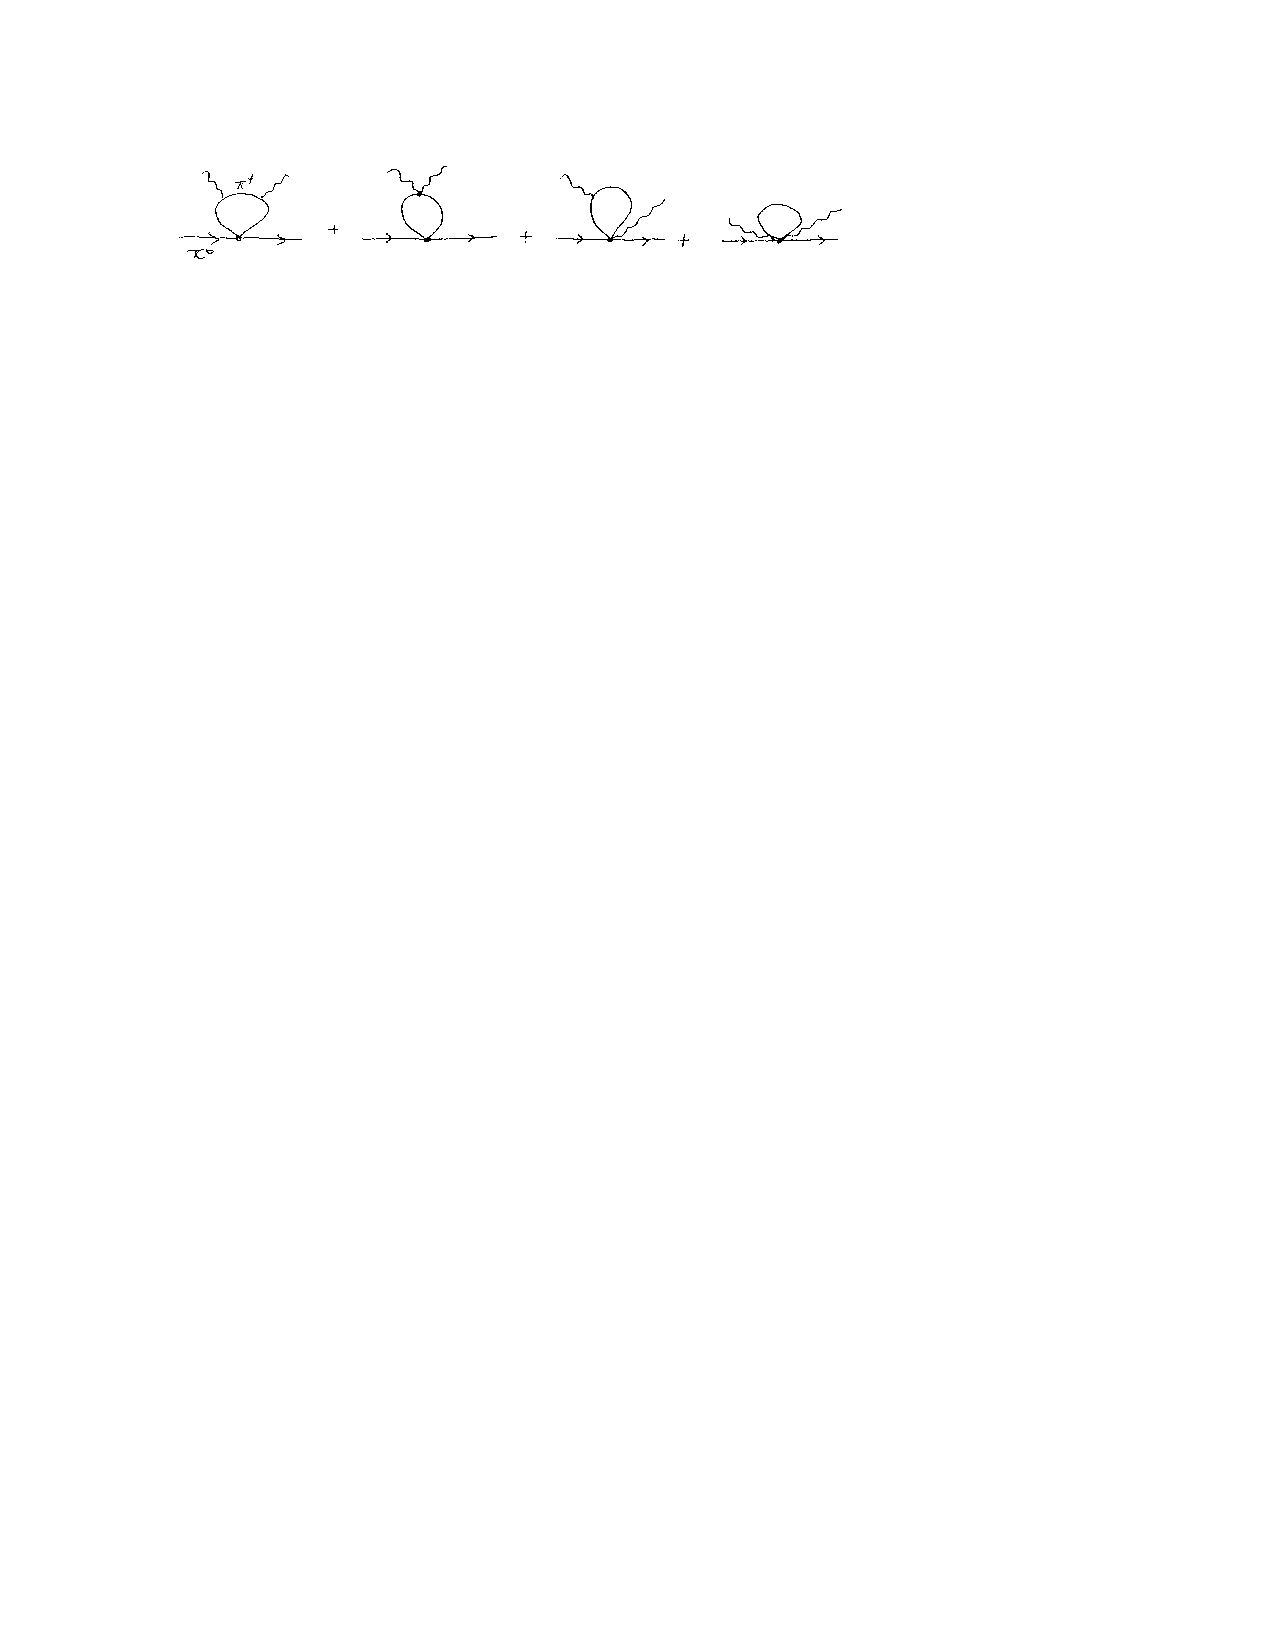
\includegraphics[height=2cm,angle=0]{figures/Fig-TP-1.pdf}
%\includegraphics[height=6cm,width=8cm,angle=0]{gA-Mpi-LHPC-band.pdf}
\end{center}
\caption{
\label{fig:digrams}}
\end{figure}


In the case of the neutral pion, the polarizabilities are determined
by the one loop chiral contributions (see Fig.\,\ref{fig:digrams})
which are calculable, free of unknown parameters, and given only in
terms of the fine structure constant, the pion mass and the pion decay
constant:
\begin{eqnarray}
\alpha_{\pi^0}+\beta_{\pi^0}&=&0\nonumber\\
\alpha_{\pi^0}-\beta_{\pi^0}&=&-\frac{\alpha}{48 \pi^2 M_\pi F_\pi^2}\simeq -1.1\times 10^{-4}~{\rm fm}^3
\end{eqnarray}
However, there is a range of predictions beyond
NLO and the experimental test of these important predictions is very
challenging. In the first place, the polarizabilities drive the very
low energy regime of Compton scattering on the $\pi^0$ as there is no
Thomson term, so one would expect that it would be easier to determine
them than in the charged pion case.  However, in the first place
Compton scattering on the $\pi^0$ is experimentally inaccessible due
to its short lifetime, and therefore it is necessary to resort to the
process of this proposal. In addition, ChPT indicates that the
polarizabilities are smaller in the case of the neutral pion, about a
third of their value for the charged pion, i.e. somewhere between
$-1.7\times 10^{-4}~{\rm fm}^3$ and $-1.9\times 10^{-4}~{\rm fm}^3$,
depending on the model. The challenge is therefore to measure the
cross section for $\gamma\gamma \to \pi^0\pi^0$ with sufficient
accuracy at low invariant mass $W_{\pi\pi}$ so that one can infer the
low-energy Compton amplitude and extract the polarizabilities. For
this purpose, the theoretical foundations have been laid in works
studying $\gamma\gamma\to \pi^0\pi^0$ both using ChPT (Bellucci et al
\cite{Bellucci:1994hx,Bellucci:1994eb}, Gasser et al
\cite{Gasser:2005ud}, Aleksejevs and Barkanova
\cite{Aleksejevs:2014eea}) and dispersion theory (Oller and Roca
\cite{Oller:2008kf}, Dai and Pennington
\cite{Dai:2014zta,Dai:2014lza}, Moussallam
\cite{Moussallam:2013una}). In particular, in ChPT at the next-to-next
to leading order, which provides the higher order quark mass
corrections to the polarizabilities, some of the low energy constants
need to be fixed and for that a significantly more accurate
measurement of the $\gamma\gamma\to \pi^0\pi^0$ cross section is
needed than available presently.

Accurate measurements of the cross section near threshold combined
with data for $W_{\pi\pi}>0.7$ GeV will provide the necessary input
for performing a full theoretical analysis, combining dispersion
theory with and without inputs from ChPT at low energy. This is a well
established method which has been used to analyze $\pi\pi$
scattering. Through such an analysis it will be possible to determine,
via combination with ChPT, the low energy Compton amplitude and
extract the polarizability combination $\alpha_\pi-\beta_\pi$. The
latter extraction represents some challenge as shown in
Fig.\,\ref{fig:previousdata}, where the polarizabilities have a small
effect on $W_{\pi\pi}$ below 0.5 GeV.  Calculations by Dai and
Pennington (Table II) \cite{Dai:2016ytz} indicate that a 1.3\%
determination of $\sigma(\gamma\gamma\rightarrow\pi^0\pi^0)$ will
determine the combination of $\alpha_{\pi^0}-\beta_{\pi^0}$ to a
precision of 10\%. The preliminary study done by Aleksejevs and
Barkanova for this proposal in relativistic ChPT with SU(3) input
indicate that sensitivity could be even better depending on specific
kinematics; the full evaluation is in progress. In general, the
determination of the accuracy one can get for $\alpha_\pi-\beta_\pi$
based on a more accurate measurement as the one proposed here is still
an issue to be further studied theoretically, with J. Goity and
A. Aleksejevs forming a group to take a lead on the project. However,
even 10\% precision would still be sufficient to difference between
various models and facilitate extraction of low-energy constants, and
thus a highly desirable result for theory.

\begin{figure}[ht]
\begin{center}
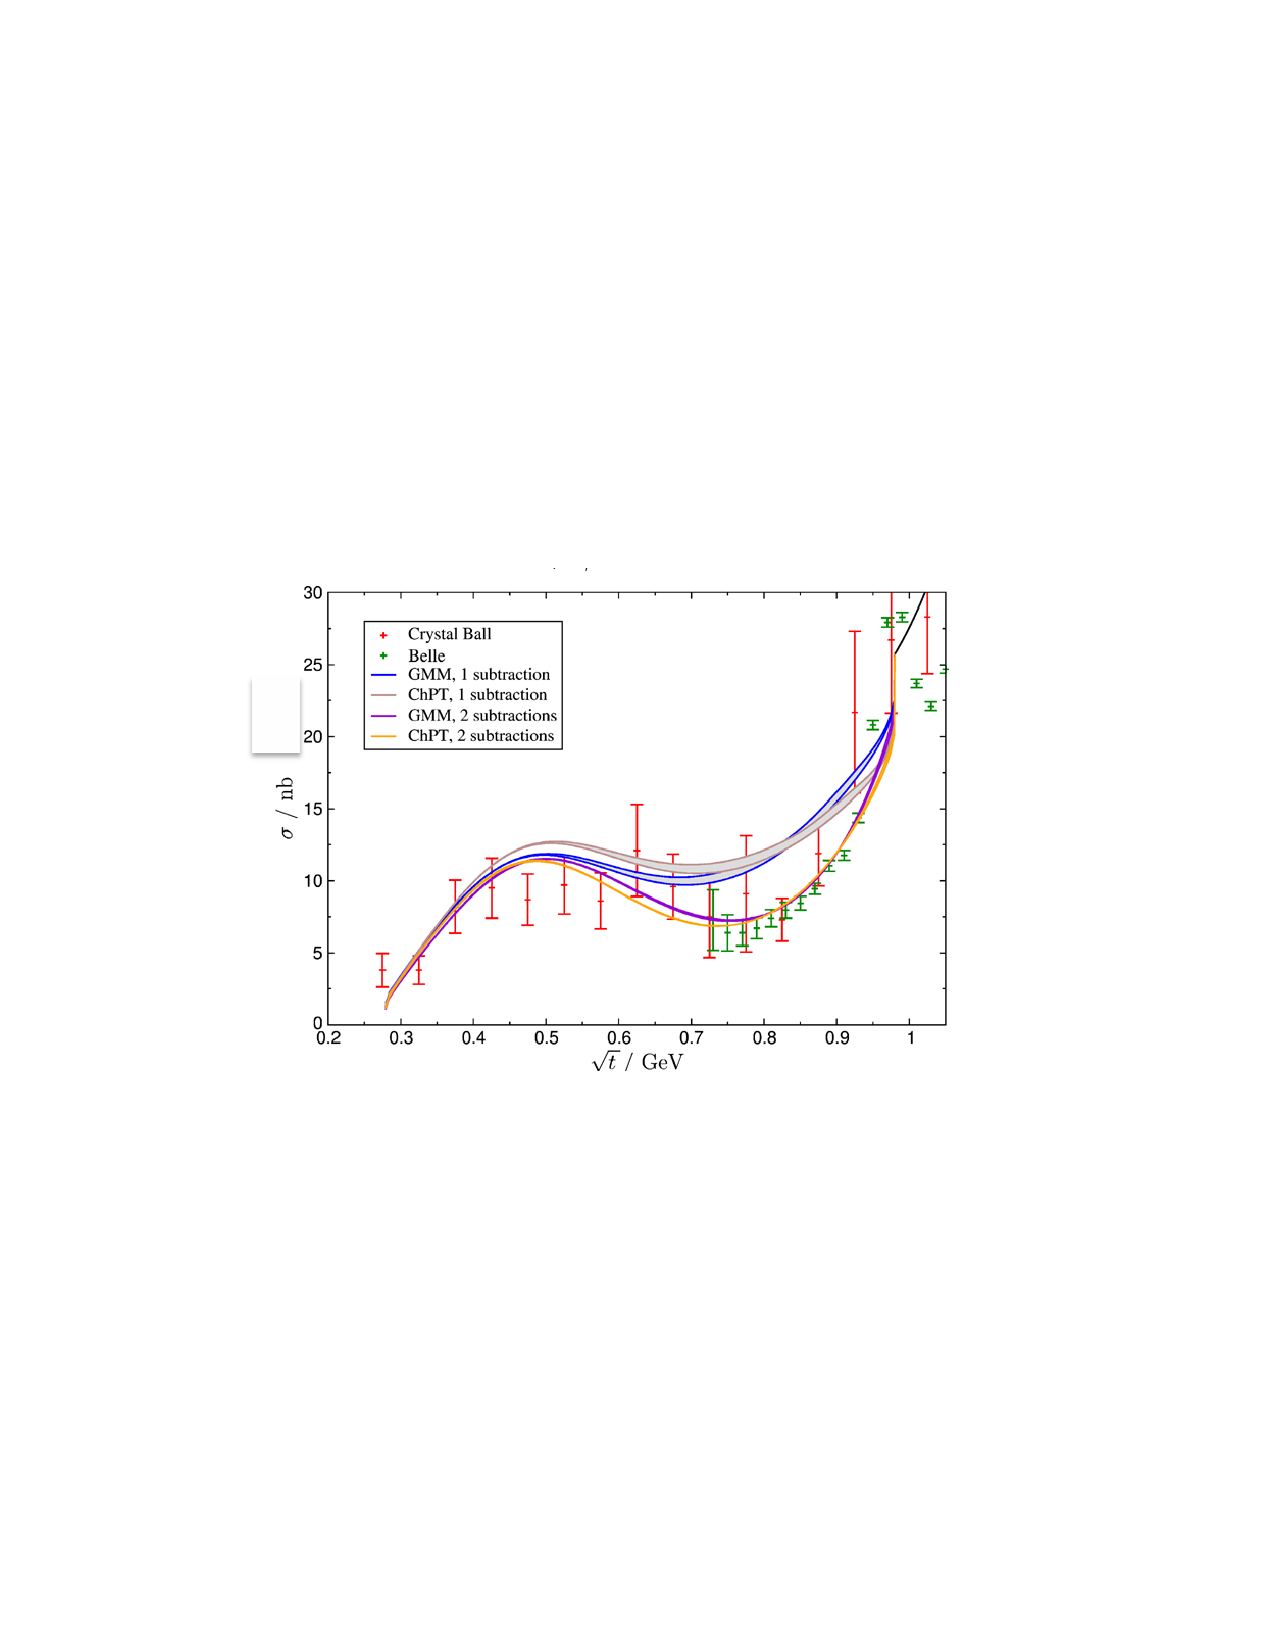
\includegraphics[height=5cm,angle=0]{figures/Fig-TP-2pr.pdf}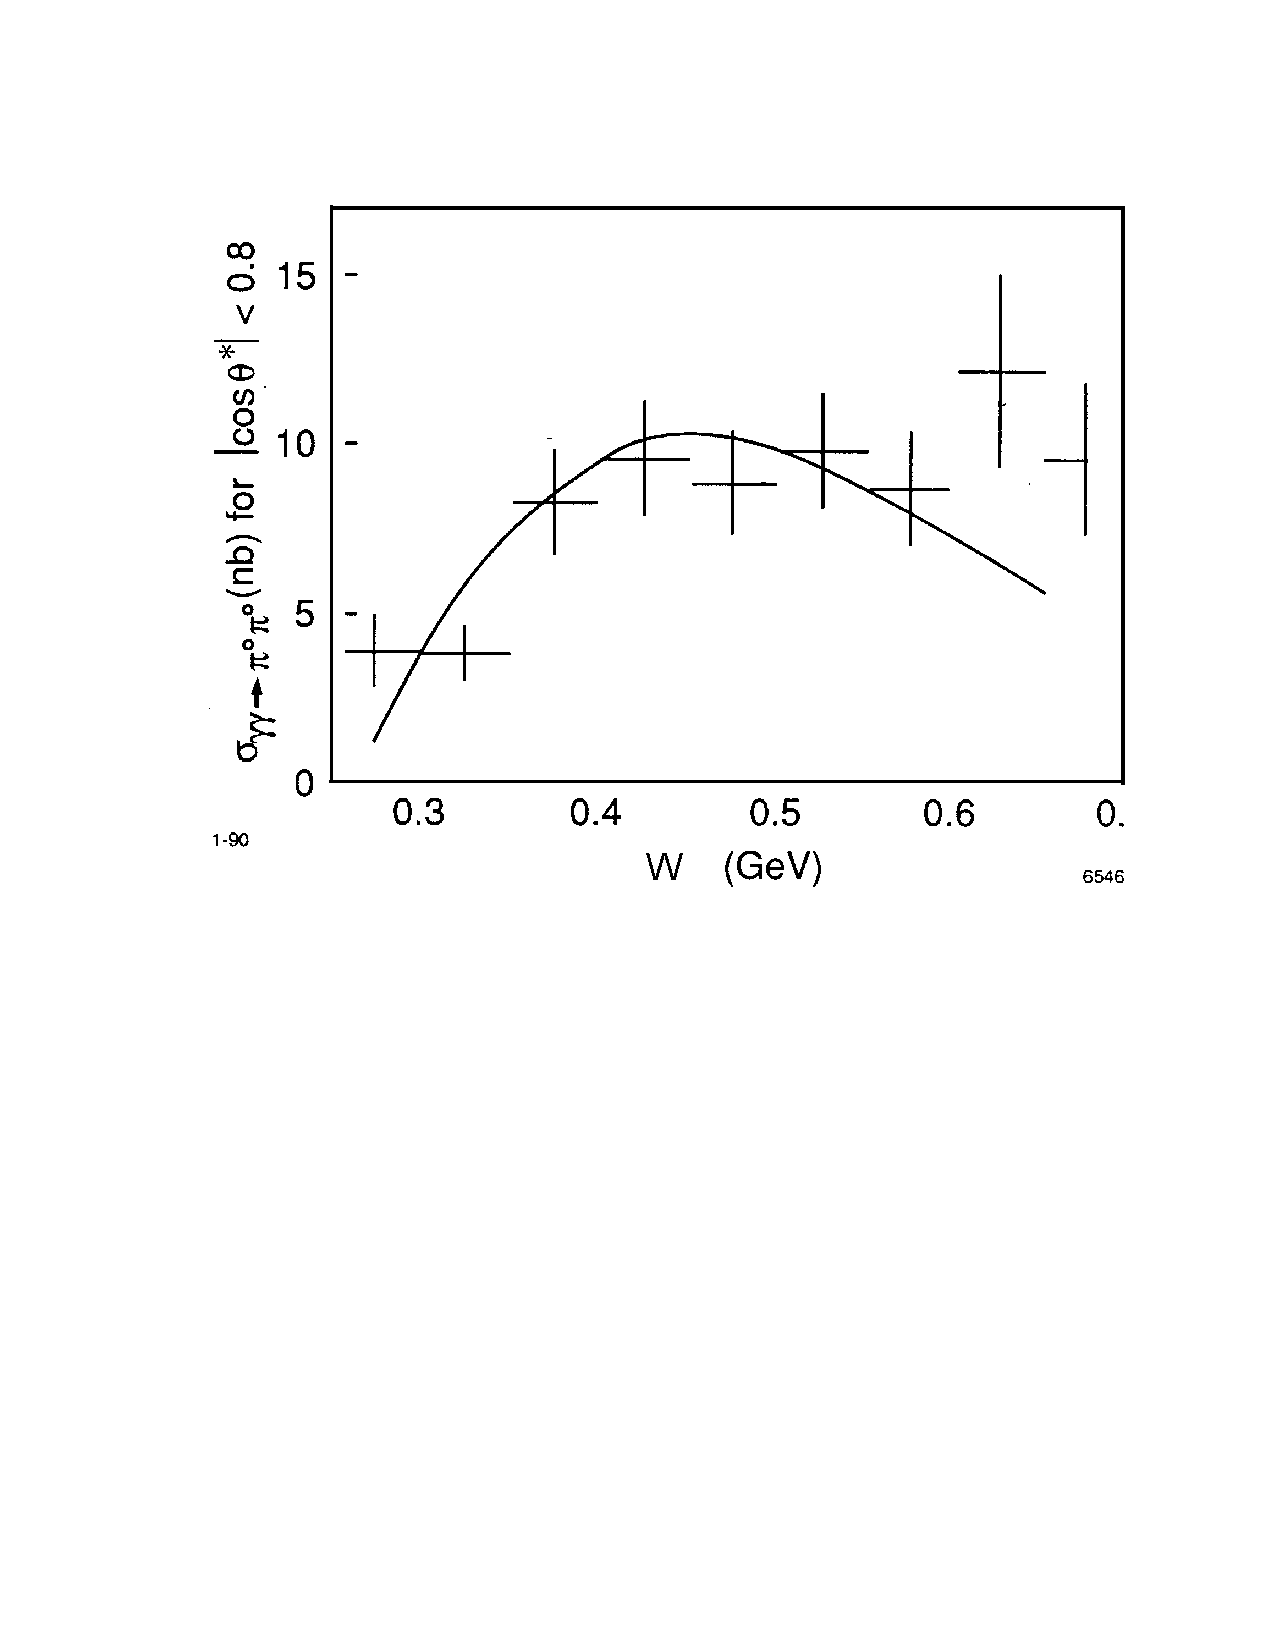
\includegraphics[height=5cm,angle=0]{figures/XBall.pdf}\\
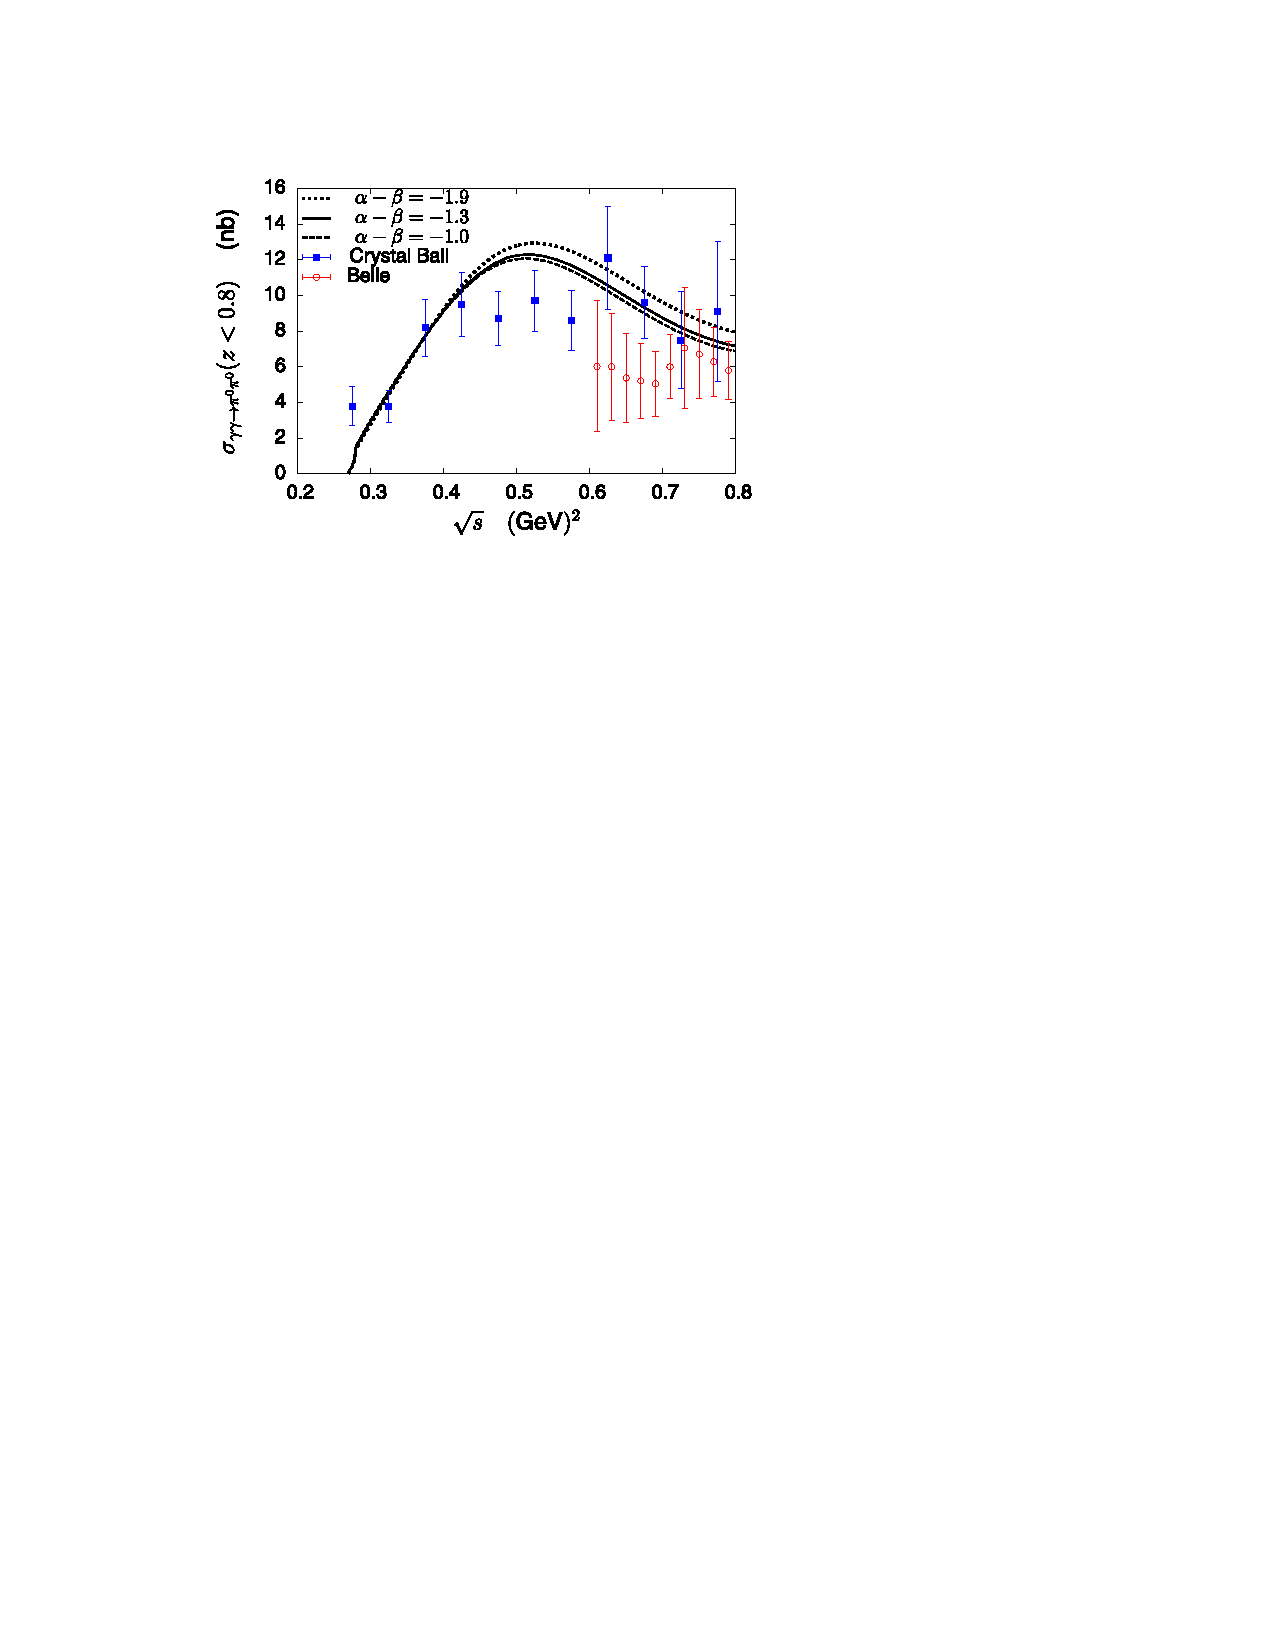
\includegraphics[height=6cm,angle=0]{figures/Fig-TP-5.pdf}\i
%\includegraphics[height=6cm,width=8cm,angle=0]{gA-Mpi-LHPC-band.pdf}
\end{center}
\caption{Left panel: experimental status; right panel: results from the 1990 XBall experiment. The lower panel shows the effect of $\pi^0$ polarizabilities on the cross section ($\sqrt{s}=W_{\pi\pi}$) \cite{Moussallam:2013una} .
\label{fig:previousdata}}
\end{figure}

\section{Past Measurements}
Past measurements of the $\gamma\gamma\to \pi^0\pi^0$ cross section can be summarized as follows:
\begin{enumerate}
    \item 
In the early 1990's measurements were made in $e^+e^-$ collisions at DESY   with the XBall detector at the DORIS-II storage ring, which are the only available data for $W_{\pi\pi}<0.6{\rm~ GeV}$ \cite{Marsiske:1990hx}. 
\item In 2008-9, measurements were carried out by BELLE
for $0.6{\rm~ GeV}<W_{\pi\pi}<4.0 {\rm~ GeV}$ \cite{Mori:2007bu,Uehara:2008ep,Uehara:2009cka}. 
\end{enumerate}
Several works have made use of dispersion theory methods (Oller and
Roca \cite{Oller:2008kf}, Dai and Pennington \cite{Dai:2016ytz}, and
in particular Moussallam \cite{Moussallam:2013una} who performed the
dispersive analysis where one of the photons has non vanishing
virtuality, which is particularly important for our case.) with those
available data. In particular these methods give results for the cross
section at small $W_{\pi\pi}$, but the poor accuracy of the data in
that region does not serve as a useful constraint that could improve
those analyses. On the other hand, the ChPT calculations carried out
at NNLO (Bellucci et al \cite{Bellucci:1994hx,Bellucci:1994eb} ) can
only be fitted to the low $W_{\pi\pi}$ data, and thus the uncertainty
in the fixing of low energy constants is rather large. It is therefore
expected that accurate data at low $W_{\pi\pi}<0.6{\rm~ GeV}$ will
have a very big impact on both theoretical approaches, which together
may allow for an accurate description of the low energy Compton
amplitude, and for a first time experimental determination of the
polarizability.


%---------------------------------------------------------------------------------------------------------------
%---------Measurements of the charged  pion polarizability-------------------------------------
%---------------------------------------------------------------------------------------------------------------
%\input{PreviousMeasurements.tex}

%---------------------------------------------------------------------------------------------------------------
%---------Measurements of the charged  pion polarizability at Jefferson Lab Hall D-----
%---------------------------------------------------------------------------------------------------------------


 %<><><><><><><><><><><><><><><><><><><><><><><><><><><><><><><><><><><><><><><><><><><><><>
 % Experimental conditions
 %<><><><><><><><><><><><><><><><><><><><><><><><><><><><><><><><><><><><><><><><><><><><><>
\section{Experimental conditions}
The measurement of the neutral pion polarizability is expected to run
concurrently with the experiment to measure the charged pion
polarizability (CPP) \cite{CPPexp} in Hall D. Essentially all the
optimizations for that experiment are expected to improve the
sensitivity of this experiment also. We briefly summarize the
configuration for CPP, which is compared in
Table\,\ref{tab:ccp_config} to nominal GlueX running.
 
The diamond radiator will be adjusted to set the coherent peak of the
photon beam between 5.5 and 6 GeV. This enhances the polarization
significantly and also the tagging ratio.  The experimental target
will be placed upstream of the nominal GlueX target by 64 cm (z=1\,cm
in the Hall D coordinate system). These changes benefit the present
experiment. In addition, the CPP experiment will add multi-wire
proportional chambers downstream for muon identification, but these do
not impact this measurement one way or another.
 
% \begin{landscape}
\begin{table}[t]
\caption{Configuration of the CPP experiment compared to nominal GlueX. This experiment is expected to run concurrently with CPP. Detectors not identified
in the table are assumed to be operated under the same conditions as in the nominal configuration.
\label{tab:ccp_config}
}
\begin{center}
\begin{tabular}{|l|c|c|c|c|c|c|c|c|}
\hline
\hline 
  Configuration  & GlueX I  & CPP   \\  \hline \hline
  Electron  beam energy  &   11.6 GeV   &  11.6 GeV   \\ \hline 
  Emittance   &   10$^{-8}$m rad   &  10$^{-8}$m rad   \\ \hline 
  Electron  current  &   150 nA   &  20 nA  \\ \hline
  Radiator thickness  &   50$\mu$m  &  50 $\mu$m diamond   \\ \hline 
  Coherent peak  &   8.4 -- 9.0 GeV   &  5.5 -- 6.0 GeV     \\ \hline 
  Collimator aperture  &  5 mm & 5 mm   \\ \hline  
  Peak polarization  &   35\%   &  72\%     \\ \hline 
  % Coherent/Incoherent ratio  &  0.068   &   0.32?   \\ \hline  
  Tagging ratio  &   0.6   &   0.72 \\ \hline  
  Flux 5.5-6.0 GeV  &      &   11 MHz \\ \hline   
  Flux 8.4-9.0 GeV  &  20 MHz    &    \\ \hline  
  Flux 0.3-11.3 GeV  &  367 MHz    &   74 MHz \\ \hline 
  Target position  &   65 cm   &  1 cm    \\ \hline 
  Target, length   &  H, 30 cm   &  $^{208}$Pb, 0.028 cm   \\
%                            &   2.1 g/cm$^2$, 0.033 X$_0$ & 0.69 g/cm$^2$, 0.05 X$_0$ \\ 
 \hline  
  Start counter & nominal & removed \\ \hline
  Muon identification  &  None   &   Behind FCAL    \\ \hline   
  \hline
\end{tabular}
\end{center}
\end{table}
%\end{

\documentclass[letterpaper,12pt]{article}

\subsection{Expected signal}
In order to estimate rates, resolution and acceptance due to the
Primakoff reaction on lead, $\gamma ^{208}\rm{Pb}\rightarrow \pi^0
\pi^0\, \rm{Pb}$, we take the reaction process to be the same as for
charged pion production and given in Eq. 8 of the Proposal for the
Charged Pion Polarizability experiment \cite{CPPexp}, which is
reproduced here for convenience:
\begin{eqnarray}
\frac{d^2\sigma}{d\Omega_{\pi\pi}dW_{\pi\pi}} = \frac{2\alpha Z^2}{\pi^2} \frac{E^4_\gamma \beta^2}{W_{\pi\pi}} \frac{\sin^2\theta_{\pi\pi}}{Q^4} |F(Q^2)|^2 \sigma(\gamma\gamma\rightarrow\pi^0\pi^0) (1+P_\gamma \cos{2\phi_{\pi\pi}}).   \label{eq:PrimakoffSignal}
\end{eqnarray}
The $\gamma\gamma$ cross section for charged pions has been
substituted with the cross section for neutral pions, namely
$\sigma(\gamma\gamma\rightarrow\pi^0\pi^0)$. In this expression,
$\Omega_{\pi\pi}$ is the solid angle in the laboratory frame for the
emission of the $\pi\pi$ system, $W_{\pi\pi}$ is the $\pi\pi$
invariant mass, Z is the atomic number of the target, $\beta$ is the
velocity of the $\pi\pi$ system, $E_\gamma$ is the energy of the
incident photon, $F(Q^2)$ is the electromagnetic form factor for the
target with final-state-interactions (FSI) corrections applied,
$\theta_{\pi\pi}$ is the lab angle for the $\pi\pi$ system,
$\phi_{\pi\pi}$ is the azimuthal angle of the $\pi\pi$ system relative
to the incident photon polarization, and $P_\gamma$ is the incident
photon polarization.\footnote{The expression for the cross section in
  terms of invariant quantities can be found in
  Ref.\,\cite{hdnote3186}.}
\begin{figure}[tph]
\centering
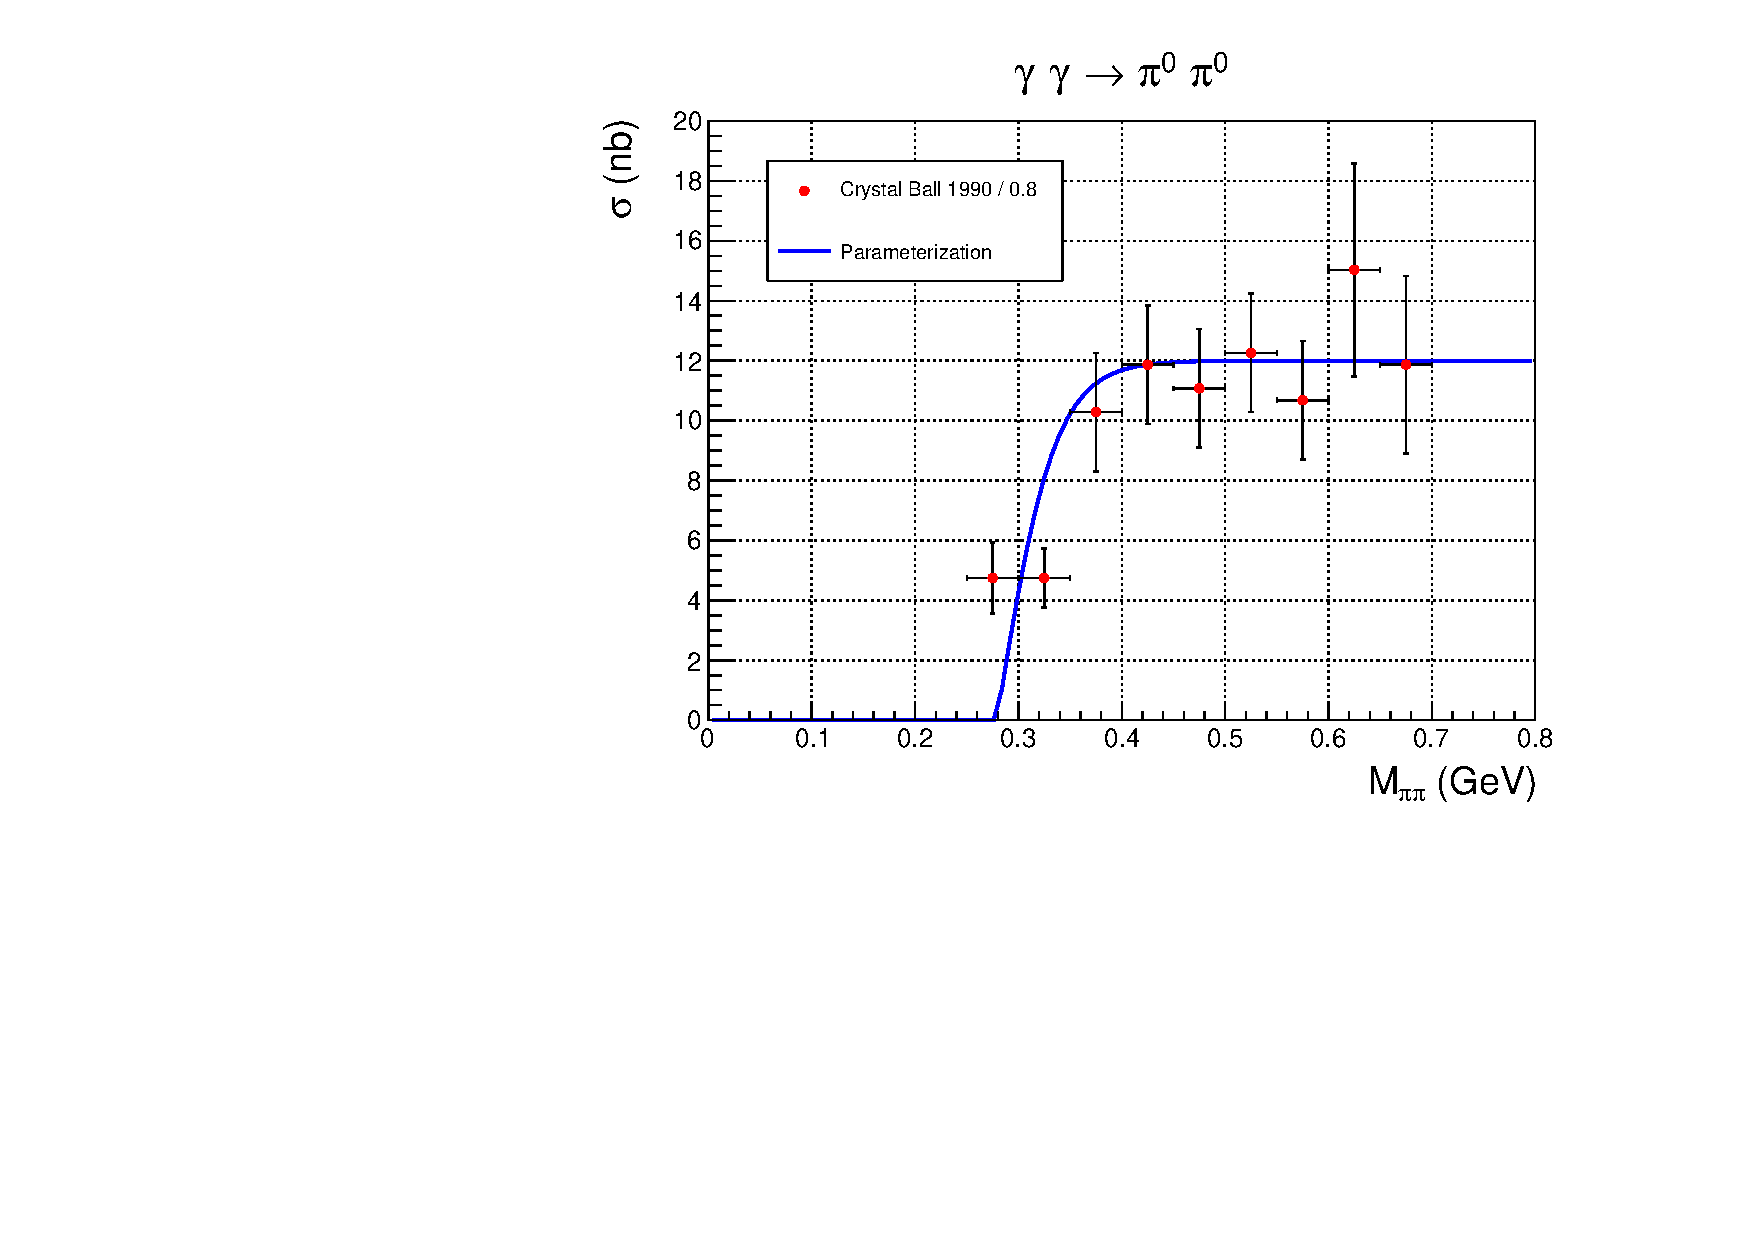
\includegraphics[page=1,width=4.75in]{figures/sigma_2pi0_figs.pdf}
\caption{Parameterization of the $\sigma(\gamma\gamma\rightarrow \pi^0\pi^0)$ cross section as a function
of the 2$\pi$ invariant mass compared to the data from Crystal Ball \cite{Marsiske:1990hx}.
\label{fig:sigma_2pi0_figs_1}}
\end{figure}

The cross section for $\sigma(\gamma\gamma\rightarrow\pi^0\pi^0)$ has
been measured by the Crystal Ball Collaboration
\cite{Marsiske:1990hx}, albeit with limited statistical precision. We
have parameterized the cross section for $W_{\pi\pi}<0.8$ GeV, which
is of specific interest to this program as shown in
Fig.\ref{fig:sigma_2pi0_figs_1}. Using this parameterization and
Eq.\ref{eq:PrimakoffSignal}, we can calculate the photoproduction
cross section on lead, which is shown in
Fig.\ref{fig:sigma_2pi0_figs_2}.
\begin{figure}[tph]
\centering
\includegraphics[page=2,width=4.75in]{figures/sigma_2pi0_figs.pdf}
\caption{Primakoff cross section for $\gamma Pb \rightarrow Pb\, \pi^0 \pi^0$ using the parameterization of  $\sigma(\gamma\gamma\rightarrow \pi^0\pi^0)$ in the previous figure. The integrated cross section is 0.3\,$\mu$b/nucleus.
\label{fig:sigma_2pi0_figs_2}}
\end{figure}
The integrated cross section is 0.30\,$\pm0.05\mu$b/nucleus. The estimated uncertainty comes from comparing two different calculations using completely different parameterizations for the nuclear form factor on lead, $F(Q^2)$. For reference,
we note that the cross section for charged pions $(\pi^+\pi^-$)
production is 10.9\,$\mu$b, a factor of 30 larger.

The number of neutral-pion-Primakoff-signal events produced during 20
PAC days is shown in Fig.\ref{fig:sigma_2pi0_figs_3}. The impacts of
detector trigger, acceptance and resolution are discussed in the next
section.
\begin{figure}[tph]
\centering
\includegraphics[page=3,width=4.75in]{figures/sigma_2pi0_figs.pdf}
\caption{Estimated production rate  for $\gamma \rm{Pb}\rightarrow \pi^0\pi^0\,\rm{Pb}$ as a function 2$\pi$ mass. For this calculation, it is assumed the detector has perfect resolution and has a linearly increasing efficiency from zero at threshold up to 0.6 at 0.34 GeV (see top right of Fig.\,\ref{fig:twopi_primakoff_DSelect_p1_W_100000_sum} ).
\label{fig:sigma_2pi0_figs_3}}
\end{figure}

\subsection{Detector resolution}
\label{sec:acceptance}
The response of the GlueX detector to neutral pion Primakoff events
was simulated using the standard GlueX generation and reconstruction
tools, but with the specific geometry for the CPP experiment. The schematic of the detector configuration is shown in
Fig.\,\ref{fig:GlueX_cpp}. The primary differences between the
standard GlueX geometry and CPP are summarized in
Table\,\ref{tab:ccp_config}. For this experiment, the main differences
include a) coherent peak position at 5.5-6 GeV and re-positioning of
the microscope to cover the coherent peak, b) solid $^{208}$Pb at
z=1cm, and c) Start counter removed. For the CPP experiment, the
addition of muon identification chambers behind the FCAL is
critical. However, for neutral pions this addition plays no role
because the photons are detected in the FCAL. The GEANT3 simulation,\footnote{The event simulation has been updated to run with GEANT4 and yields similar results.}
which is used for these studies, includes most changes except for the
addition of the muon chambers, which are not needed. In addition, the
microscope geometry has not been modified and we use the tagger
hodoscope for that region in the simulation. The slightly reduced
energy of the hodoscope relative to the microscope has little impact
and the gaps between counters is ignored by simulating the tagged
flux.
\begin{figure}[h!]
\centering
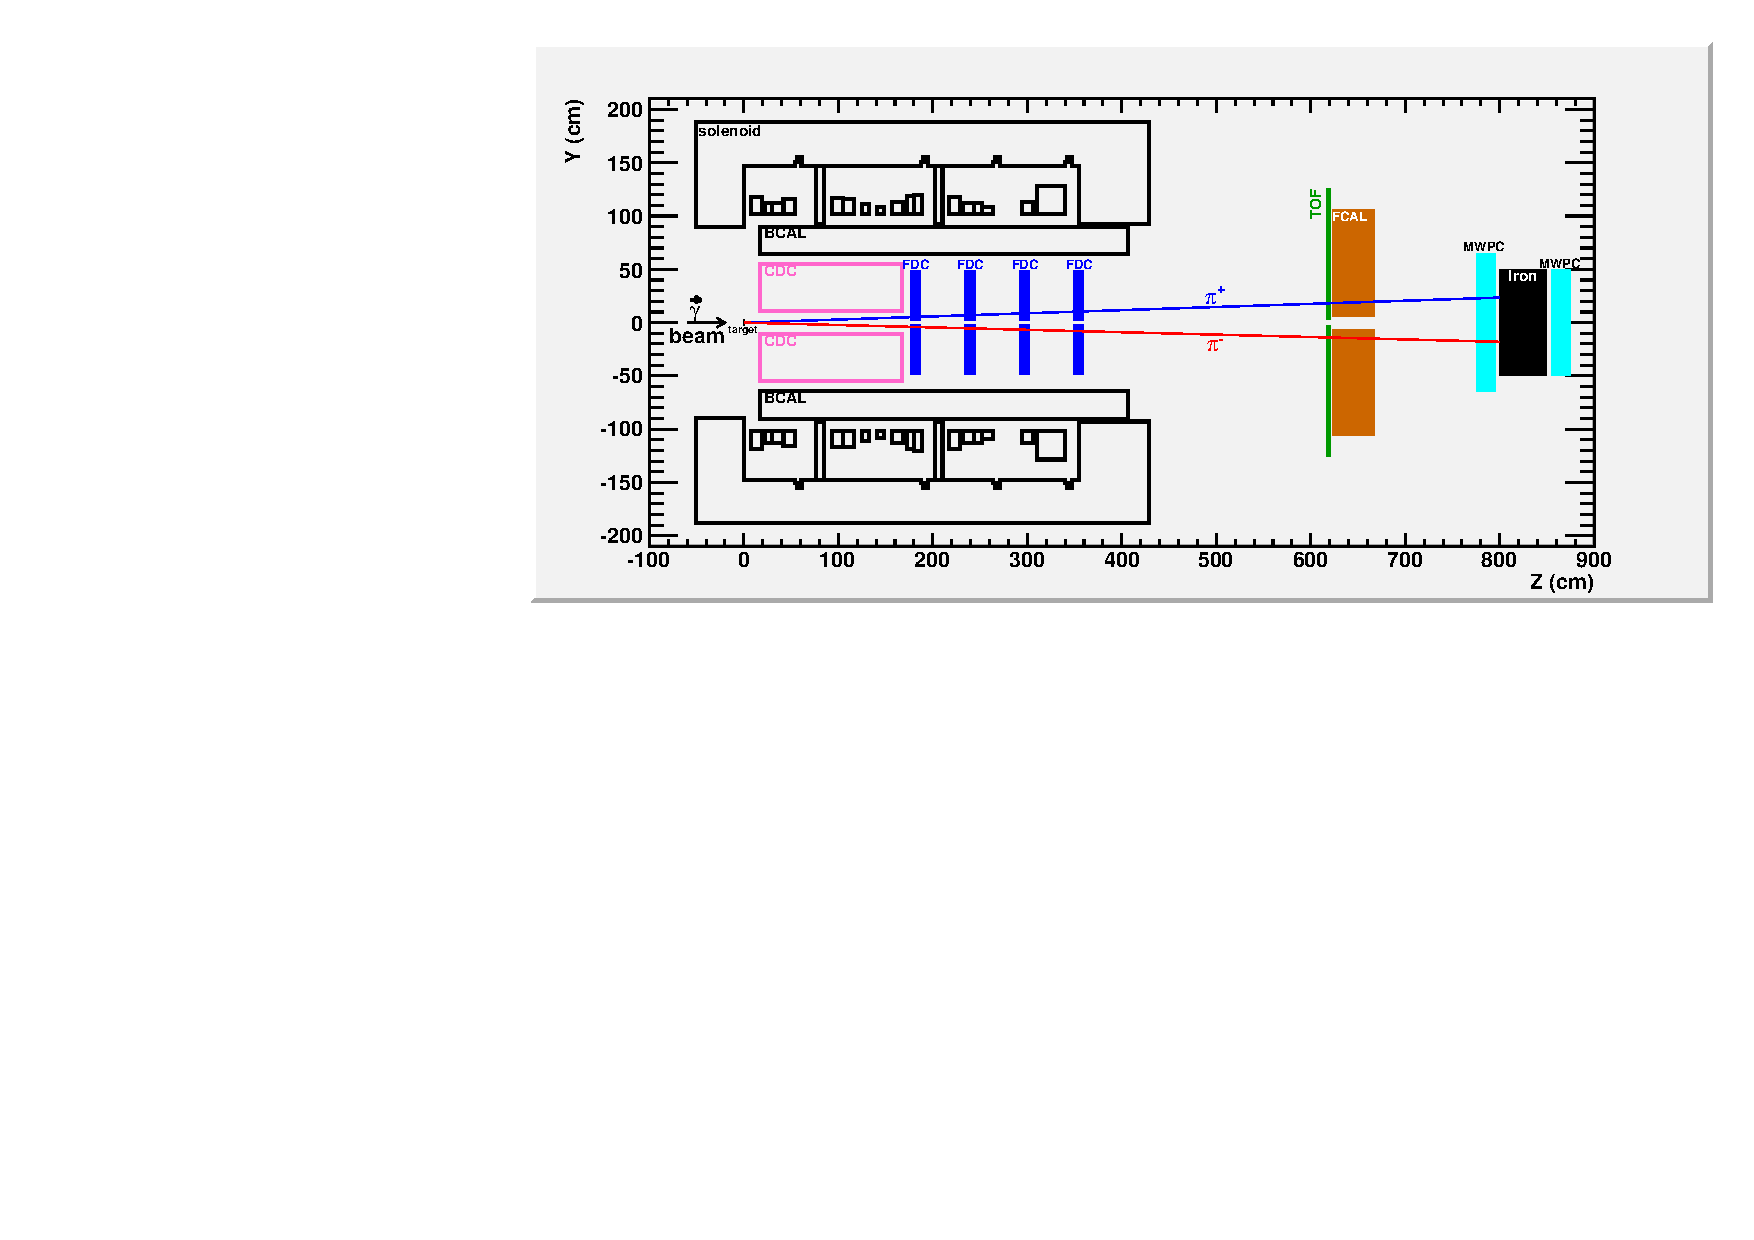
\includegraphics[width=5.25in]{figures/GlueX_cpp.pdf}
\caption{Diagram of the GlueX detector including the additional muon chambers for the CPP experiment.}
\label{fig:GlueX_cpp}
\end{figure}

The Primakoff signal was generated according to the cross section
described in the previous chapter, using the
\emph{gen\_2pi0\_primakoff}, which is a modified version of the CPP event generator. By default, the production amplitudes are
symmetrized between the two identical $\pi^0$'s by AmpTools. One
hundred thousand events were generated with $M_{\pi\pi}<$0.5 GeV and
with no background, fed to GEANT3 to track particles, and subsequently
processed using \emph{mcsmear} to simulate the detector response. The
simulated events were then analyzed using the GlueX event filter to
analyze the reaction $\gamma Pb \rightarrow \pi^0 \pi^0$ with a
missing Pb nucleus and constraining the detected photon pairs to the
$\pi^0$ mass. Energy and momentum conservation is imposed on the reaction as well as the requirement that all photons originate from a common vertex (i.e. ``vertex-P4''). The output of the reconstruction, both kinematically
fit and ``measured" quantities, were available for inspection.

In the following we show various reconstructed quantities as well as
estimated resolutions. The distribution of generated photon energy and
the unconstrained reconstructed momenta of the two pions are shown in
Fig.\,\ref{fig:EgP1P2_signal_DSelector}.
\begin{figure}[tph]
\centering
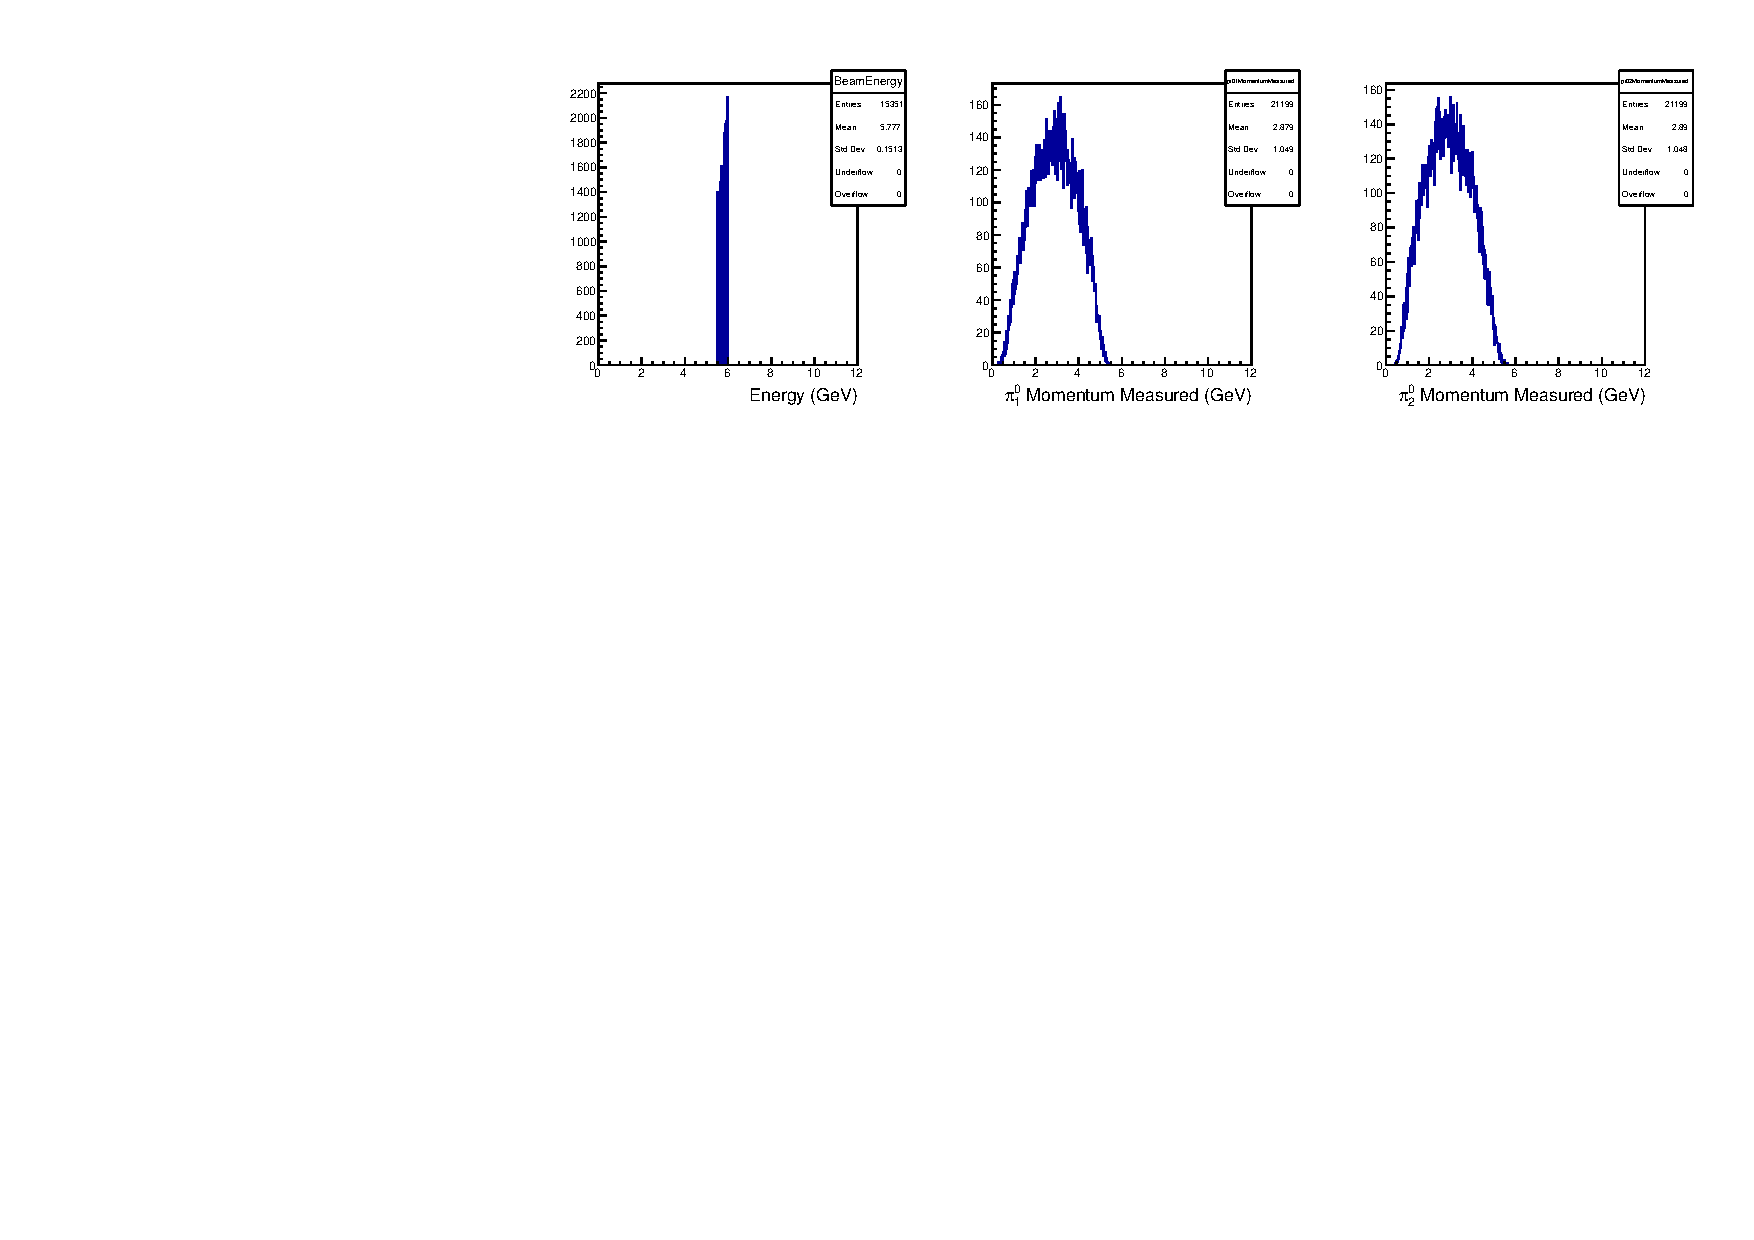
\includegraphics[width=6in]{figures/EgP1P2_signal_DSelector.pdf}
\caption{Left: Generated photon energies. Center: Reconstructed momentum distribution of one $\pi^0$. Right: Reconstructed momentum distribution of the second $\pi^0$.
\label{fig:EgP1P2_signal_DSelector}}
\end{figure}
The missing mass, 2$\pi$ mass and $-t$ distributions are shown in Fig.\,\ref{fig:MMMpipit_signal_DSelector}.
\begin{figure}[tph]
\centering
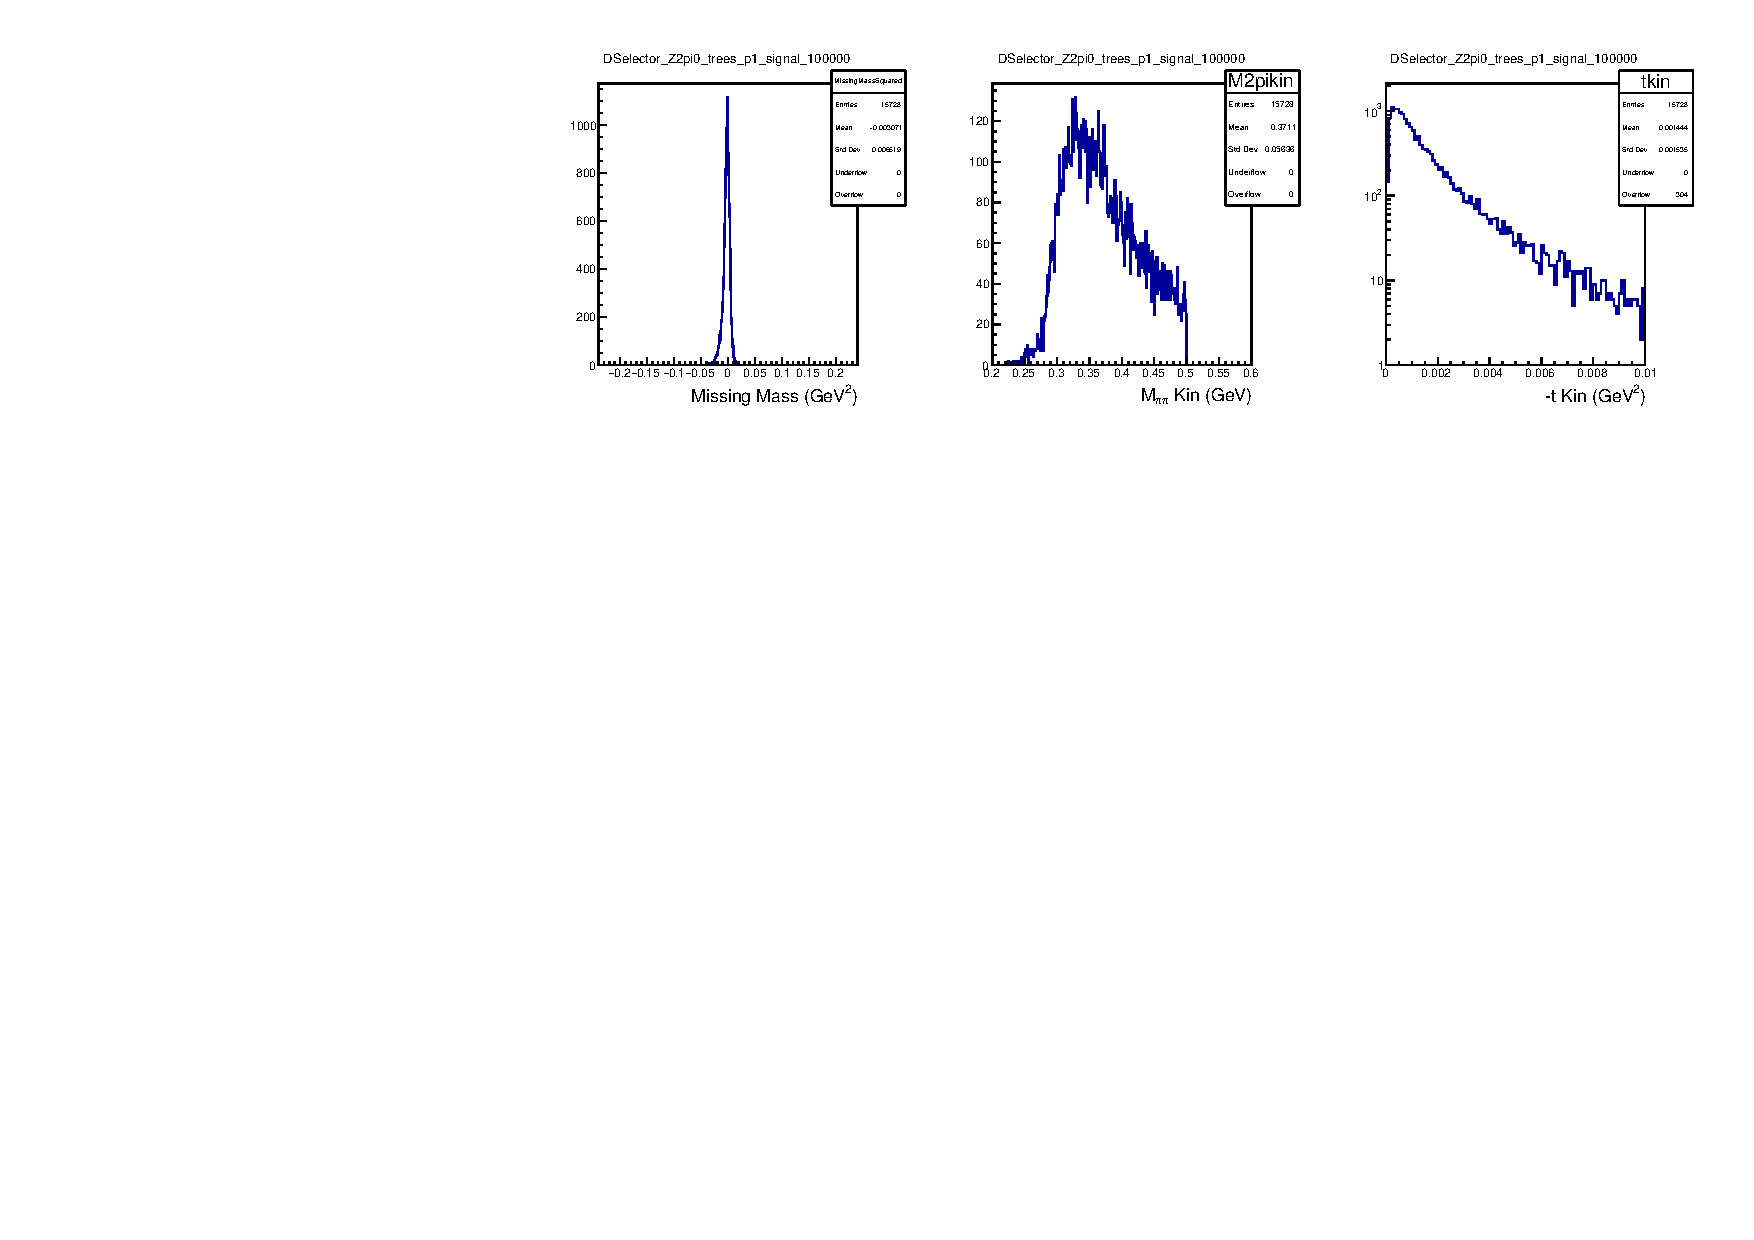
\includegraphics[width=6in]{figures/MMMpipit_signal_DSelector.pdf}
\caption{Left: Missing mass distribution minus the mass of the recoil nucleus. Center: Kinematically fit $2\pi$ mass distribution. Right: Kinematically fit -t distribution.
\label{fig:MMMpipit_signal_DSelector}}
\end{figure}
The reconstructed momentum relative to its generated value is shown in
Fig.\ref{fig:DeltapDeltaPhi_signal_DSelector}. The central peak of the
kinematicall fit momentum is about 2\%, similar to that for charged
pions. However, there are long uniform tails that will effect the
final reconstruction. The resolution of the azimuthal angle,
$\phi_{\pi\pi}$, between the production and the photon polarization
planes is quite poor owing to the fact that the pion pairs are
produced at very shallow angles. Nevertheless it is sufficient to
measure the asymmetry due to the photon beam polarization.
\begin{figure}[tph]
\centering
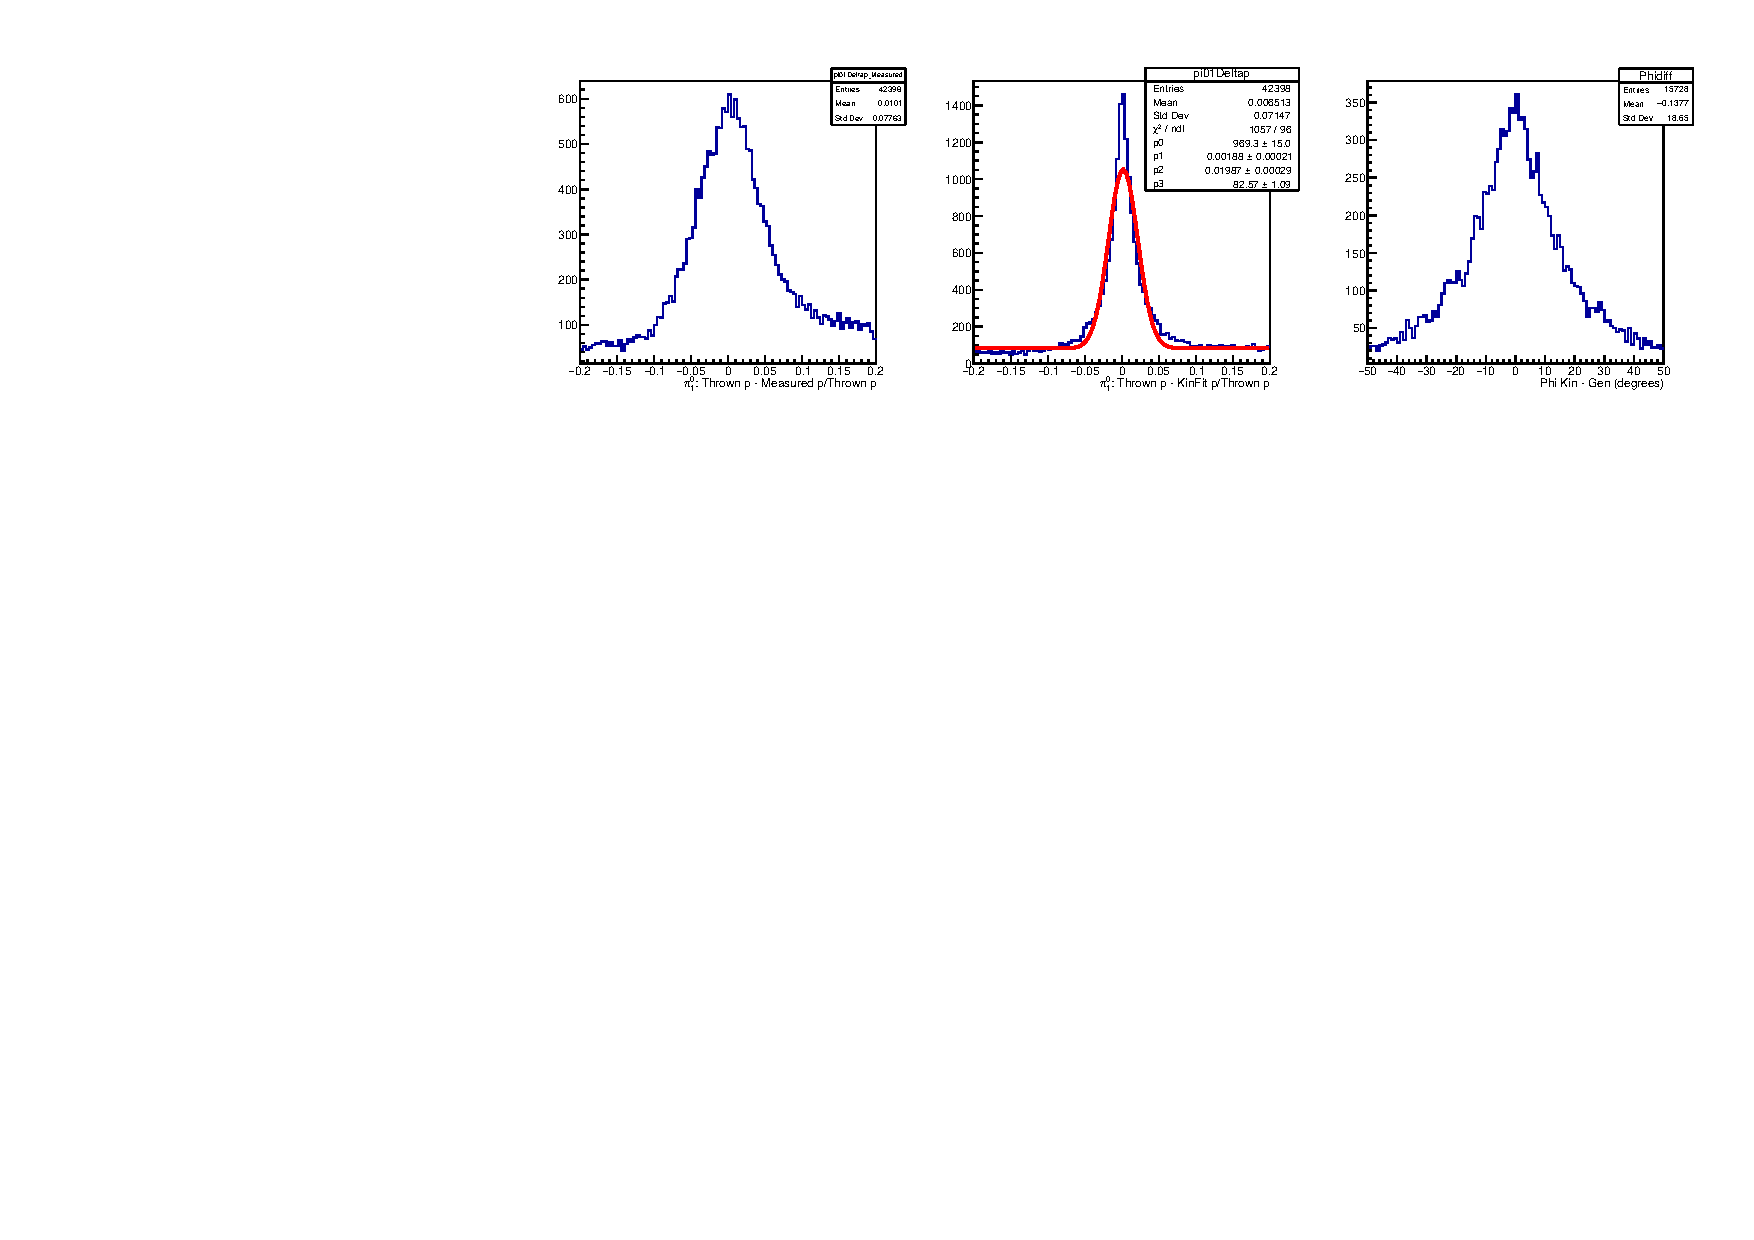
\includegraphics[width=6in]{figures/DeltapDeltaPhi_signal_DSelector.pdf}
\caption{Left: Difference between measured and generated momentum. Center: Difference between kinematically fit and generated momentum. The central peak has a width of about 2\%. Right: Difference between the kinematically fit azimuthal angle $\phi_{\pi\pi}$ and its generated value.
\label{fig:DeltapDeltaPhi_signal_DSelector}}
\end{figure}
The resolution of the 2$\pi$ invariant mass is shown in Fig.\,\ref{fig:Resolution_Mpipittag_signal_DSelector}, along with the resolution of Mandelstam $-t$, and the reconstructed time resolution. The mass resolution is about 8\,MeV.
\begin{figure}[tph]
\centering
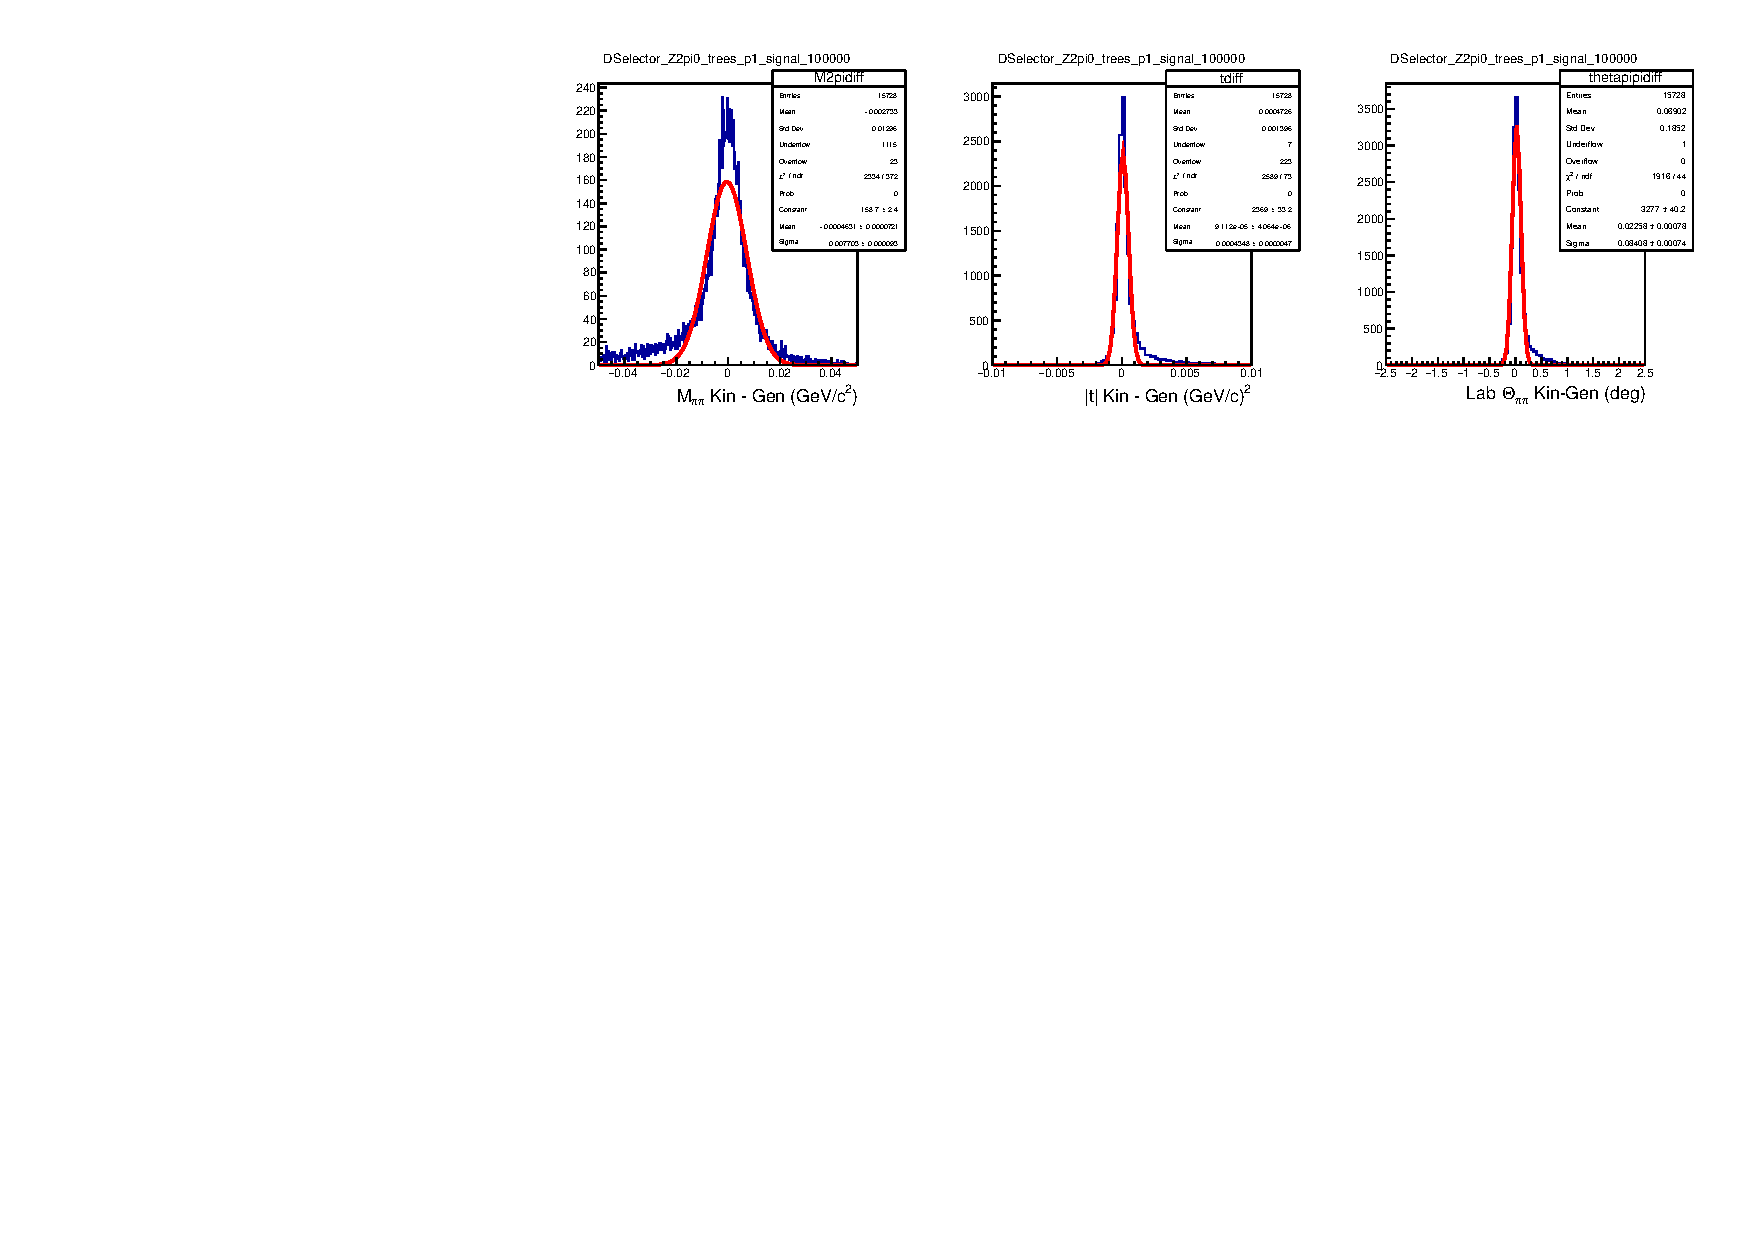
\includegraphics[width=6in]{figures/Resolution_Mpipittag_signal_DSelector.pdf}
\caption{Left: Difference between kinematically fit and generated 2$\pi$ mass. The central 2$\pi$-mass $\sigma$ is about 8 MeV. Center: Difference between kinematically fit and generated -t. Right: Difference between kinematically fit and generated 2$\pi$ polar angle. The resolution $\sigma$ of the reconstructed angle is less than 0.1 degrees.
%Right: Timing resolution relative to the accelerator RF signal is about 0.35 ns.
\label{fig:Resolution_Mpipittag_signal_DSelector}}
\end{figure}

\subsection{Trigger and acceptance}
The Primakoff reaction will transfer all the energy of the beam into
four photons, which are going forward. All this energy will be
deposited in the FCAL, except for leakage down the beampipe. We expect
a simple trigger with an energy threshold in the FCAL should have very
high efficiency for any events that can be reconstructed.

The acceptance of the signal events can be determined by comparing the
kinematically fit to the generated distributions. The generated and
kinematically fit 2$\pi$ mass, $\phi_{\pi\pi}$ and $-t$ distributions
are shown in
Fig.\,\ref{fig:twopi_primakoff_DSelect_p1_W_100000_sum}. The
reconstruction was described in the previous section.
\begin{figure}[tph]
\centering
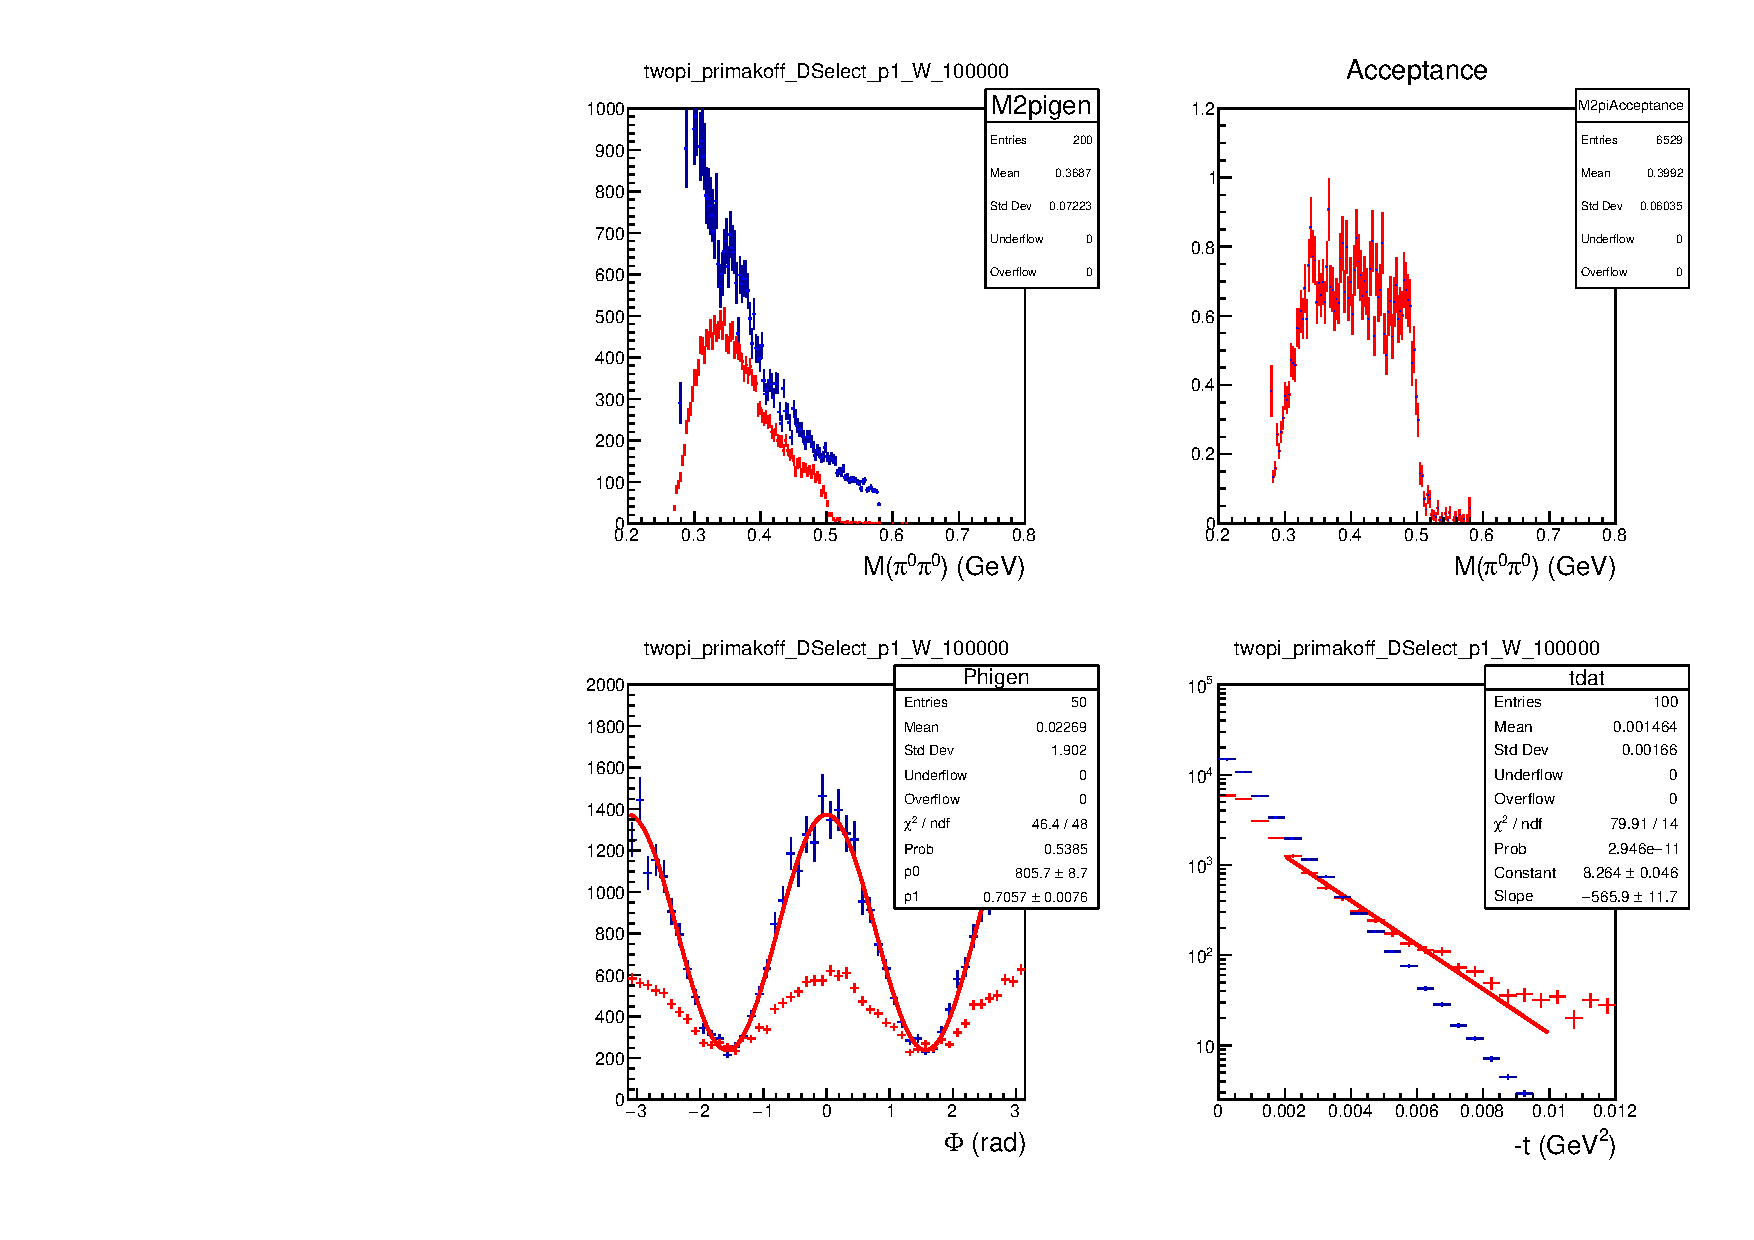
\includegraphics[width=6in]{figures/twopi_primakoff_DSelect_p1_W_100000_sum.pdf}
\caption{Top left: Generated and kinematically fit 2$\pi$ mass distribution. Top right: Acceptance as a function of 2$\pi$ mass. Events above $M_{\pi\pi}>$0.5 GeV were eliminated from the analysis. The acceptance is about 60\%. Bottom left: Generated and kinematically fit azimuthal angle $\phi_{\pi\pi}$. Bottom right: Generated and kinematically fit $-t$ distribution. There is significant slewing of the measured distribution to large $-t$.}
\label{fig:twopi_primakoff_DSelect_p1_W_100000_sum}
\end{figure}
The acceptance is quite high at about 60\%. However, there is also
significant slewing due to resolution in most variables of
interest. The main effect of resolution in the 2$\pi$ mass happens at
threshold and the distortions above that are not very great. The
relatively poor resolution in $\phi_{\pi\pi}$ results in dilution of
the measured azimuthal dependence, which will need to be adjusted
based on simulation. Finally the $-t$ resolution softens the measured
t-slope due to the smearing of high rate regions down to low rate
regions.


%<><><><><><><><><><><><><><><><><><><><><><><><><><><><><><><><><><><><><><><><><><><><><>
 % Backgrounds
 %<><><><><><><><><><><><><><><><><><><><><><><><><><><><><><><><><><><><><><><><><><><><><>
\subsection{Backgrounds}

\subsubsection{Coherent and incoherent backgrounds in the reaction}

Coherent $\rho^0$ photo-production is not a background for this
experiment because $\rho^0$ decay into the $\pi^0\pi^0$ channel is
prohibited by I-spin conservation.  The largest coherent background is
from $f_0(500)$ and $f_0(980)$ photo-production.  The width of the
$f_0(980)$ is from 10 to 100~MeV, and can be eliminated from the data
by a cut on $\pi^0\pi^0$ invariant mass.  The $f_0(500)$ width is much
broader, from 400 to 700 MeV, with significant overlap in the
invariant mass region of interest.  Since the $f_0(500)$ is a scalar
particle with the same spin-parity as the $\gamma \gamma \rightarrow
\pi^0\pi^0$ final state near threshold, the azimuthal distribution of
the $\pi^0$ momentum or the $\pi^0\pi^0$ c.m. momentum relative to the
photon polarization plane does not differentiate between coherent
$f_0(500)$ production and the Primakoff reaction.  This is similar to
the Primex-$\pi^0$ experiment, where the dominant background was
nuclear coherent $\pi^0$ photo-production.  The approach used in the
Primex analysis was to measure the $\pi^0$ angular distribution,
effectively the $t$-distribution, then use theoretical calculations of
the angular distributions to separate out contributions from Primakoff
and nuclear coherent. The analysis of the $\pi^0\pi^0$ (NPP) reaction
will approximately parallel what was done for the Primex-$\pi^0$
analysis.

Primex data also showed that the nuclear coherent process is highly
suppressed for heavy nuclei.  The reason for the suppression is
$\pi^0$ absorption in the nuclear interior, making the coherent
production primarily a surface effect, i.e. proportional to $A$ and
not $A^2$.  For NPP it is expected that suppression of the nuclear
coherent will be stronger than that seen in Primex because two pions
are produced in NPP as compared to a single $\pi^0$ in Primex.  NPP
plans to run on a heavy nuclear target such as $^{208}$Pb.

The inelastic and incoherent reactions that might contribute to the
data include
\begin{enumerate}[label=(\roman*)]
    \item nuclear coherent production of $\eta$ followed by $\eta\rightarrow \pi^0\pi^0\pi^0 \rightarrow \gamma\gamma\gamma\gamma(\gamma\gamma)$, where two of the six decay photons go unobserved
    \item $\gamma N \rightarrow N \pi^0\pi^0$
\end{enumerate}

The first reaction is an inelastic, coherent process, and as such
could produce a significant rate for a heavy nuclear target. Rejecting
events with extra gammas in the final state would suppress this
background.  The second reaction is an incoherent process, and is
small relative to coherent processes.  The Primex analysis showed that
incoherent reactions generally peak at large angles relative to the
Primakoff peak, and had a small effect on the extraction of the
Primakoff $\pi^0$ cross sections.
\section{Photon beam flux}

\subsection{Photon beam flux accounting with the GlueX pair spectrometer}
The photon beam flux can be directly extracted by analyzing the pair
spectrometer (PS) data with the thin beryllium converter installed in
the beam in from of it.  The absolute normalization of the PS
performed with the total absorption counter (TAC) during the dedicated
run.

The systematics from the photon beam flux accounting by pair
spectrometer is originated from few main contributions: overall
spectrometer calibration with TAC quality; accuracy of the Monte-Carlo
simulation of this process; long term stability of the spectrometer
performance; and change of conditions between low intensity beam (TAC
calibration) and production intensity.  There are few other less
significant contributions. GlueX PS acceptance \cite{hdnote3684} shown
on Fig.~\ref{fig:psacc}. For the proposed experiment PS magnetic field
should be reduced to cover the beam energy range $5-6\,GeV$.
\begin{figure}[tpb]
\begin{center}
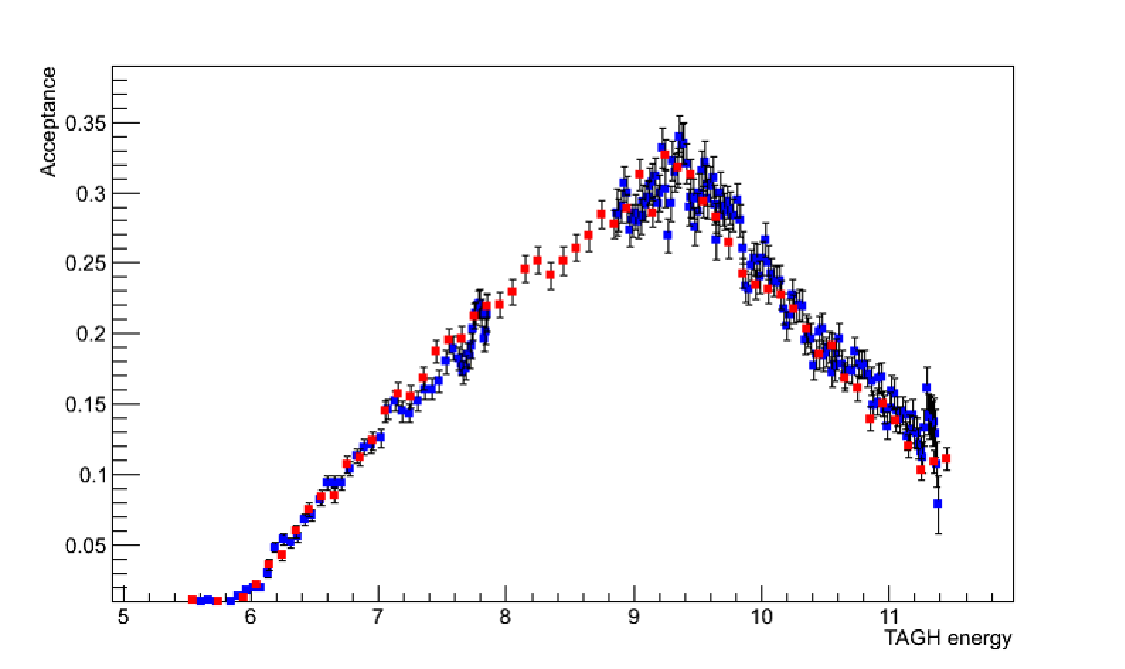
\includegraphics[width=10cm,angle=0]{figures/ps_acceptance.pdf}
\end{center}
\caption{GlueX PS acceptance extracted from TAC data analysis (blue points);
red points -- Monte-Carlo simulation}
\label{fig:psacc}
\end{figure}
The methodology and accuracy of the PS analysis is the same as in
PrimEx-D experiment, currently running in Hall-D, and has value
$\sim1-1.5\,\%$ \cite{PrimexDexp}.

\subsection{Cross section verification with the exclusive single $\pi^0$ photoproduction}
The extracted cross section can also be normalized on or independently
from PS analysis verified with the $\pi^0$ radiative decay width
extraction.  Fig.~\ref{fig:leaddndt} shows exclusive single $\pi^0$
photoproduction yield at forward angle obtained by the PrimEx
experiment and used for $\pi^0$ radiative decay width extraction.
\begin{figure}[tpb]
\begin{center}
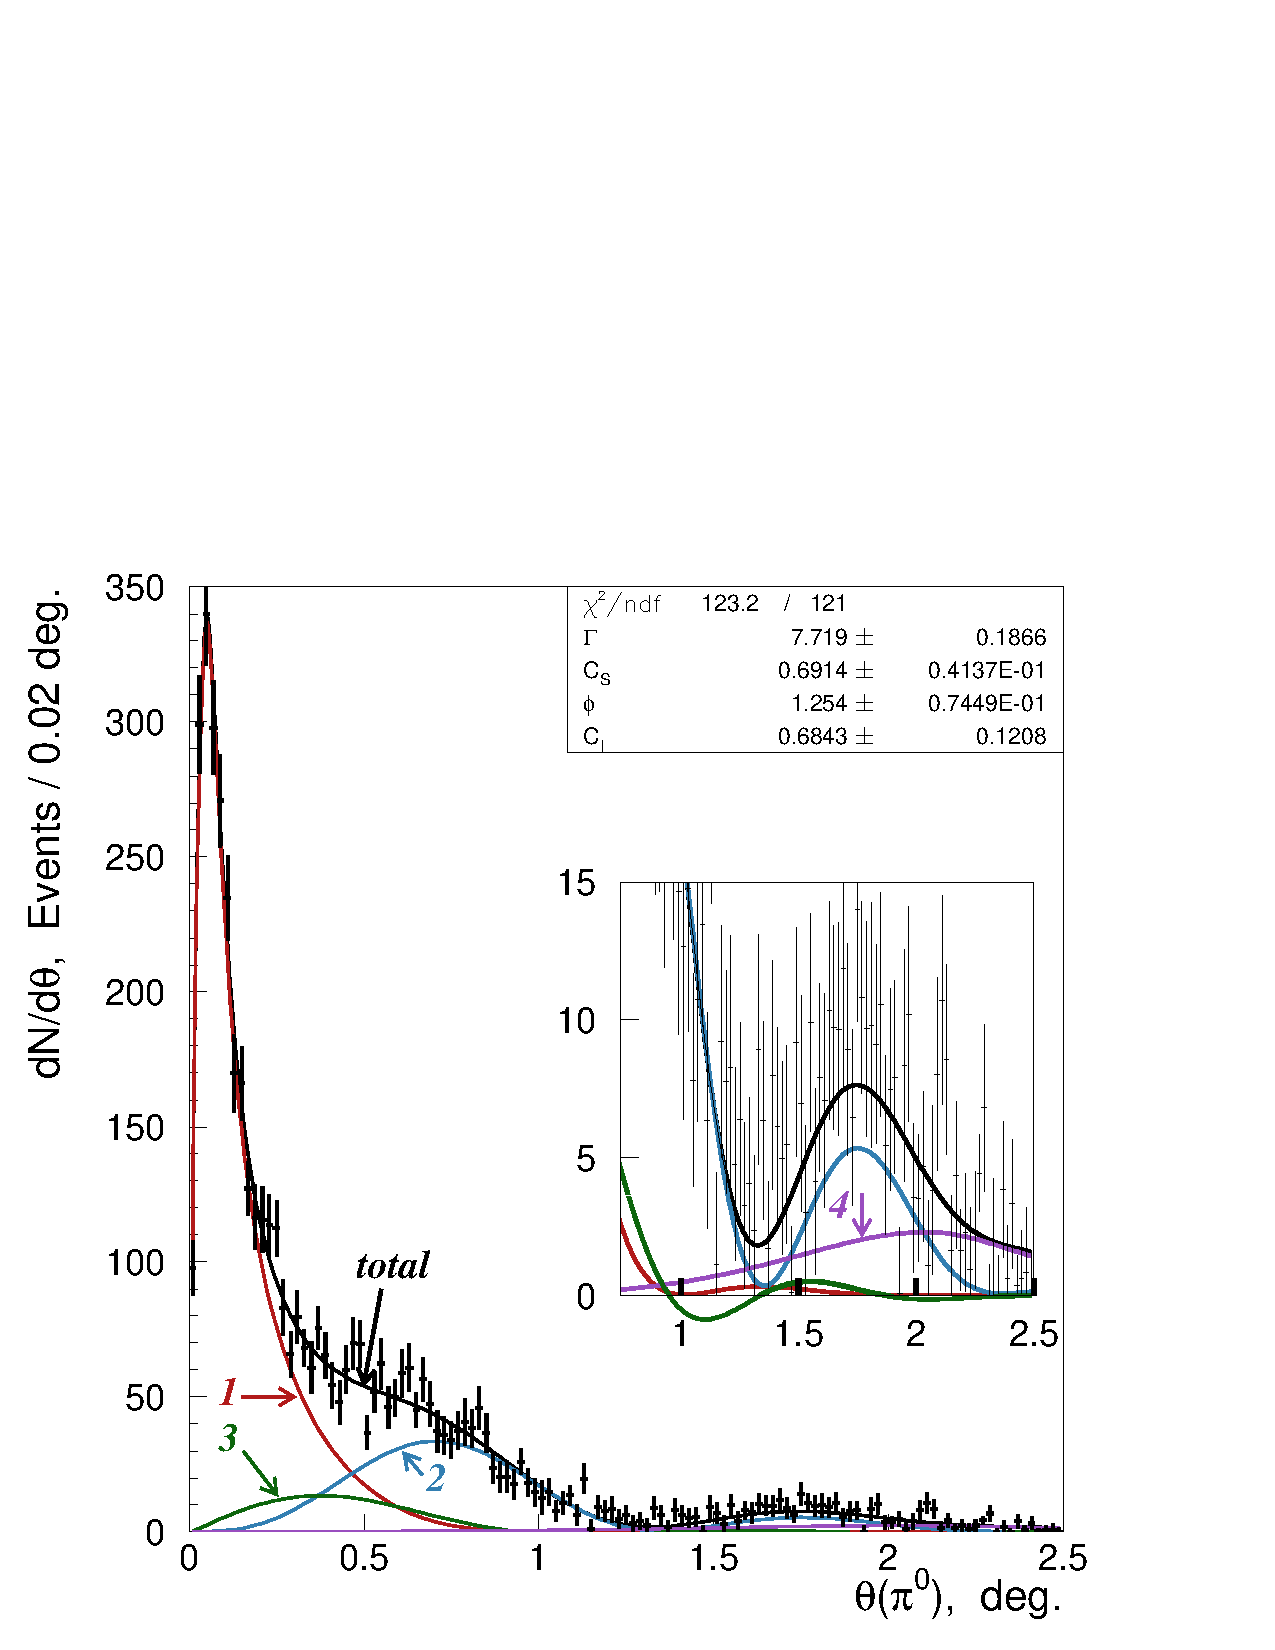
\includegraphics[width=8cm,angle=0,trim={1.5cm 0.5cm 3.5cm 9.5cm},clip]{figures/dndt_pb_partial.pdf}
\end{center}
\caption{Exclusive $\pi^0$ production yield at forward angle on lead target
observed in the PrimEx experiment \cite{Larin:2010kq}. Curves show production mechanisms input:
1 -- Primakoff, 2 -- strong coherent, 3 -- interference of first two mechanisms, 4 -- strong incoherent}
\label{fig:leaddndt}
\end{figure}
The photon beam flux in PrimEx was $0.725\times10^{12}$ for
4.9-5.5$\,$GeV bremsstrahlung spectrum part on 5\% rad. len. lead
target. The distance between calorimiter and target was $\sim7.3\,m$
and the central square part of the calorimeter, used in analysis was
$\sim70\times70\,cm$. These conditions have to be compared with the
proposed experiment conditions: 20 days of $~10^7$ collimated beam
photon/sec (i.e. 20 times more than PrimEx lead target beam flux), the
distance between target and FCAL $\sim6.2\,m$ and active calorimeter
part diameter $\sim2\,m$.  The central hole with one calorimeter
modules layer around which should be excluded from the analysis for
PrimEx case was $\sim8\times8\,cm$ and for FCAL $\sim20\times20\,cm$,
which is decreasing FCAL acceptance at forward angle. Comparison of
these experimental conditions allows us expecting an order of
magnitude higher exclusive single $\pi^0$ photoproduction statistics.
Thus PrimEx statistical uncertainty for lead will be decreased from
$\sim2.5\,\%$ down to $\sim1\,\%$.  For the systematical uncertainty,
in PrimEx it was $\sim2.1\,\%$ and has two major contributions: yield
extraction ($\sim1.6\,\%$) and photon beam flux accounting
($\sim1.0\,\%$).  The first contribution is partly statistically
driven and reduces with increasing of statistics; and the second one
cancels out since it is the same photon beam flux for the single and
double exclusive $\pi^0$ photoproduction.  The main factors increasing
systematics for the proposed experiment are: the angular resolution of
FCAL is about a factor of two worse than for PWO crystals used in the
PrimEx analysis;
%the single $\pi^0$ photoproduction theory needs to be involved since
%the photon beam energy spectra are not the same for PrimEx and
%proposed experiment;
and the magnetic field is not swiping out charged background like it
was in PrimEx.  As a result we can expect slightly worse systematical
uncertainty than in PrimEx and statistical precision of $\sim1\,\%$,
i.e. total error $2.5-3.5\,\%$ for $\pi^0$ radiative width extraction
(excluding absolute photon beam flux accounting, target number of
atoms and partly FCAL trigger efficiency contributions to the
systematics which are canceling out).  The expected total beam flux
uncertainty for such a normalization should also include the PrimEx
total error of the $\pi^0$ radiative width, which was recently
reported as 1.5\% \cite{Larin:2018}.  All this gives $\sim3-4\,\%$
error for photon beam flux from normalization to the re-exctracted
$\pi^0$ radiative decay width.

\subsection{Muon pair production}
In addition to these normalization channels, production of muon pairs,
which has a known cross section, can be used as a measurement of
photon flux. Since the experiment will be running concurrently with
the Charged Pion Polarizability (CPP) experiment, the photon flux on
target will be the same by definition. CPP plans to use muon pair
creation by beam photons as its main normalization channel, and so
those measurements will be available for normalization of the neutral
pion channel as well. In the case of CPP, the GlueX track finding and
fitting efficiency will have to be determined for muon pairs, but any
systematic error in that determination will largely cancel when
applied to charged pion pairs. That will not be the case for the
neutral pion channel and will have to be taken into account when
evaluating systematic errors due to this method of normalization. In
any case, muon pair production should provide a useful check on the
other methods mentioned above.

\section{Errors and Sensitivity}
We summarize the anticipated errors in the determination of the $\pi^0$ polarizability. We assume 
20 days of running on a 5\% radiation length $^{208}$Pb target, 10$^7$ photons/s, and nominal acceptance for $\pi^0 \pi^0$.
Table \ref{errors} summarizes the estimated statistical and systematic errors. In the following we describe each of
these contributions in detail: 

%\end{landscape}
% \begin{landscape}
\begin{table}[bt]
\caption{Uncertainties in the extraction of $\pi^0$ polarizabilities $\alpha_{\pi^0}-\beta_{\pi^0}$.
\label{errors}
}
\begin{center}
\begin{tabular}{|l|l|c|c|}
\hline
\hline
  &  Source  & Uncertainty   \\  \hline \hline
  1 & Signal extraction  &  5 \%    \\ \hline
  2 & Flux normalization &  1.5 \%     \\ \hline
  3 & Background subtraction  & $<$1 \%  \\ \hline
  4 & Detector acceptance and efficiency &  3.5 \%   \\ \hline
  5 & Total systematic error  &  3.9\% \\ \hline
  6 & Total error on cross section  &  6.3\% \\ \hline
  7 & Projected error in $\alpha - \beta$ &  49\%  \\ 
 \hline
 \hline
\end{tabular}
\end{center}
\end{table}
%\end{landscape}

\begin{enumerate}

\item
Primakoff signal extraction from the angular distribution (Fig.\,\ref{fig:fit_Primakoff_sigma}), which also contains nuclear coherent contributions to the cross section. This uncertainty
is approximately 5\%.

\item
Flux normalization. We have several methods for determining the flux (Section\,\ref{sec:flux}). The Primex-D experiment expects an uncertainty of 1.5\% and we use that as our estimate here.

\item
Subtraction of backgrounds other than nuclear coherent. These backgrounds are not expected to be significant ($< 1\%$) and studies are on-going. 

\item
Detector acceptance and efficiency. We can measure the detector acceptance times efficiency for the process $\gamma \mathrm{Pb} \rightarrow \pi^0 \mathrm{Pb}$ with an accuracy of 3.5\% (Section\,\ref{sec:pi0norm}), which
should allow us to reduce the systematic uncertainty in the acceptance calculation for the process of interest to this level.

\item
Total systematic error (items 2-4): combining the systematic errors in quadrature gives 3.9\%.

\item 
Error on cross section (quadrature sum of items 1 and 5): 6.3\%.

\item
The current estimate by Dai and Pennington (Table II in Ref.\,\cite{Dai:2016ytz}) indicates
that a 13\% determination of
$\sigma(\gamma\gamma\rightarrow\pi^0\pi^0)$ will determine the
combination $\alpha_{\pi^0}-\beta_{\pi^0}$ to a precision of 100\%, i.e., $\Delta(\alpha_{\pi^0}-\beta_{\pi^0}) \sim 7.7\Delta(\sigma$) .
From here we estimate that our uncertainty on $\Delta(\alpha_{\pi^0}-\beta_{\pi^0}) \sim$ 49\%. We note that the basis for extracting the polarizabilities may be improved
in the near future and theoretical effort is being directed specifically toward this goal.

\end{enumerate}

\begin{table}[hbt]
\caption{Approved beam request and running conditions for CPP. NPP would run concurrently.
\label{request}
}
\begin{center}
\begin{tabular}{|l|c|c|c|c|c|c|c|c|}
\hline
\hline
  Running condition  &            \\ \hline
  Days for production running  &   20   \\ \hline
  Days for calibrations &  5       \\ \hline
  Target   & $^{208}$Pb   \\ \hline
  Photon intensity in coherent peak &   10$^7$ photons/s     \\ \hline
  Edge of coherent peak  &  6 GeV   \\ \hline
 \hline
 \hline
\end{tabular}
\end{center}
\end{table}
 
\section{Summary and beam request}
We have investigated the possibility of determining the neutral pion
polarizabilities $\alpha_{\pi^0}-\beta_{\pi^0}$, a quantity for which there are no existing measurements.
Our proposal is to extract the polarizability from a 
measurement of the cross section of the Primakoff reaction $\gamma
\rm{Pb}\rightarrow \pi^0 \pi^0 \rm{Pb}$. We propose to make this
measurement using data taken simultaneously with the CPP\cite{CPPexp}
experiment in Hall D. Table \ref{request} summarizes the approved beam request for the CPP experiment.
The existing GlueX detector has sufficient
resolution and high acceptance for this process. We expect to collect approximately 2500 signal events during the
approved 20 PAC days. The anticipated statistical uncertainties on
the signal represent a significant improvement over existing data as shown in Fig.\,\ref{fig:sigma_2pi0_figs_4}.
Using the estimate by Dai and Pennington \cite{Dai:2016ytz} we expect to be able to make the first extraction of the 
$\alpha_{\pi^0}-\beta_{\pi^0}$ polarizability with an uncertainty of 49\%.

\begin{figure}[tpb]
\centering
\includegraphics[page=4,width=4.75in]{figures/sigma_2pi0_figs.pdf}
\caption{Estimated statistical uncertainties on determining $\sigma(\gamma\gamma\rightarrow\pi^0\pi^0$) during 20 PAC days running simultaneously with the approved CPP experiment. The data points from the single previous Cristal Ball measurement \cite{Marsiske:1990hx} are shown for comparison.
\label{fig:sigma_2pi0_figs_4}}
\end{figure}






%\input{JLAB_MuonDetector.tex}



%---------------------------------------------------------------------------------------------------------------
%--------------------------------- References-----------------------------------------------------------------
%---------------------------------------------------------------------------------------------------------------
\clearpage

%\nocite{*}
\bibliographystyle{unsrt}                                                                              
\bibliography{Pi0Polarizability}   


\end{document}
